\documentclass[a4paper,twoside]{article}

\usepackage{epsfig}
\usepackage{subfigure}
\usepackage{calc}
\usepackage{amssymb}
\usepackage{amstext}
\usepackage{amsmath}
\usepackage{amsthm}
\usepackage{multicol}
\usepackage{pslatex}
\usepackage{apalike}
\usepackage{SciTePress}
\usepackage[small]{caption}

\subfigtopskip=0pt
\subfigcapskip=0pt
\subfigbottomskip=0pt

\begin{document}

\title{FlexRender: A distributed rendering architecture for ray tracing huge scenes on commodity hardware.}

\author{\authorname{Bob Somers\sup{1} and Zo\"{e} J. Wood\sup{1} }
\affiliation{\sup{1}California Polytechnic  University, San Luis Obispo, CA, USA}
\email{bob@bobsomers.com, zwood@calpoly.edu}
}

\keywords{Rendering, cluster computing, distributed rendering}

\abstract{As the quest for more realistic computer graphics marches steadily on,
the demand for rich and detailed imagery is greater than ever. However, the
current ``sweet spot'' in terms of price, power consumption, and performance
is in commodity hardware. If we desire to render scenes with tens or hundreds
of millions of polygons as cheaply as possible, we need a way of doing so that
maximizes the use of the commodity hardware that we already have at our disposal.
Techniques such as normal mapping and level of detail have attempted to address
the problem by reducing the amount of geometry in a scene. This is problematic
for applications that desire or demand access to the scene's full geometric
complexity at render time. More recently, out-of-core techniques have provided
methods for rendering large scenes when the working set is larger than the
available system memory. We propose a distributed rendering architecture based
on message-passing that is designed to partition scene geometry across a cluster
of commodity machines in a spatially coherent way, allowing the entire scene to
remain in-core and enabling the construction of hierarchical spatial acceleration
structures in parallel. The results of our implementation show roughly an order
of magnitude speedup in rendering time compared to the traditional approach,
while keeping memory overhead for message queuing around 1\%.
}

\onecolumn \maketitle \normalsize \vfill

\begin{figure}[h!]
    \centering
    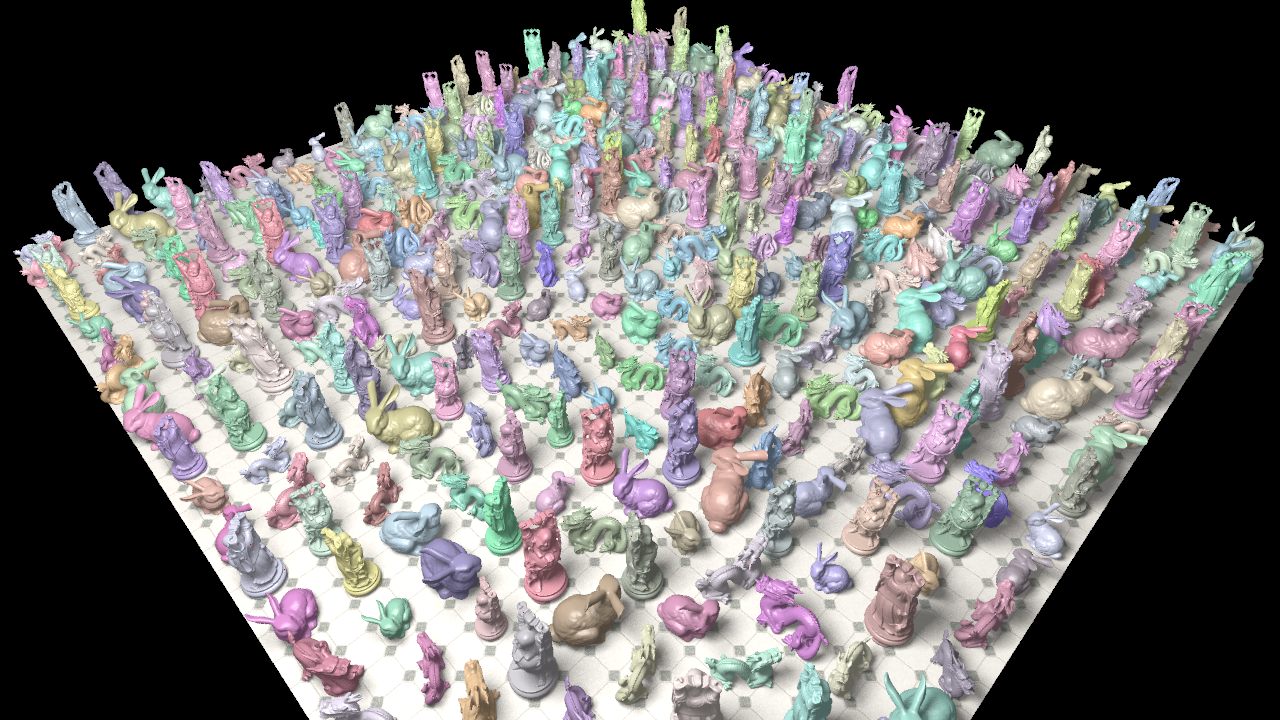
\includegraphics[width=80mm]{showoff/field.png}

    \caption{Field of high resolution models. The geometric complexity is nearly 87 million triangles.}
    \label{fig:sofield}
\end{figure}

\section{\uppercase{Introduction}}
Rendering has advanced at an incredible pace in recent years. At the heart of
rendering is describing the world we wish to draw, which has traditionally been
done by defining surfaces. While exciting developments in volume rendering
techniques happen on a regular basis, it is unlikely we will abandon surface
rendering any time soon. Unfortunately for volumes, algorithms that operate on
them are inherently $n^3$.

The champion of surface representations in rendering, has been the polygonal
mesh. Meshes are efficient to process and easy for artists to work with because
they represent discrete points in space and the connectivity between those
points (rather than abstract equations). However, their core advantage is also
their core drawback. Because everything is defined explicitly, meshes with fine
levels of detail have significantly higher storage requirements. Thus, as the
demand for higher visual fidelity increases, the natural tendency is to increase
geometric complexity.

Graphics, and ray tracing in particular, has long been said to be a problem that
is \emph{embarrassingly parallel}, given that many graphics algorithms operate
on pixels independently. Graphics processing units (GPUs) have exploited this
fact for years to achieve amazing throughput of graphics primitives in real-time.
While processor architectures have become exceedingly parallel and posted
impressive speedups, the memory hierarchy has not had time to catch up. For a
processor to perform well, the CPI, \emph{cycles per instruction}, must remain
low to ensure time is spent doing useful work and not waiting on data.

In current memory hierarchies, data access time can take anywhere from around
12 cycles (4 nanoseconds for an L1 cache hit) to over 300 cycles (100
nanoseconds for main memory). Techniques such as out-of-order execution are
helpful in filling this wasted time, but for memory intensive applications it
can be difficult to fill all the gaps with useful work. Thus, keeping the chips
``hot'' by reducing time spent waiting on data is critical to achieving maximum
performance, and is an extremely challenging problem.

\begin{figure}[h!]
    \centering
    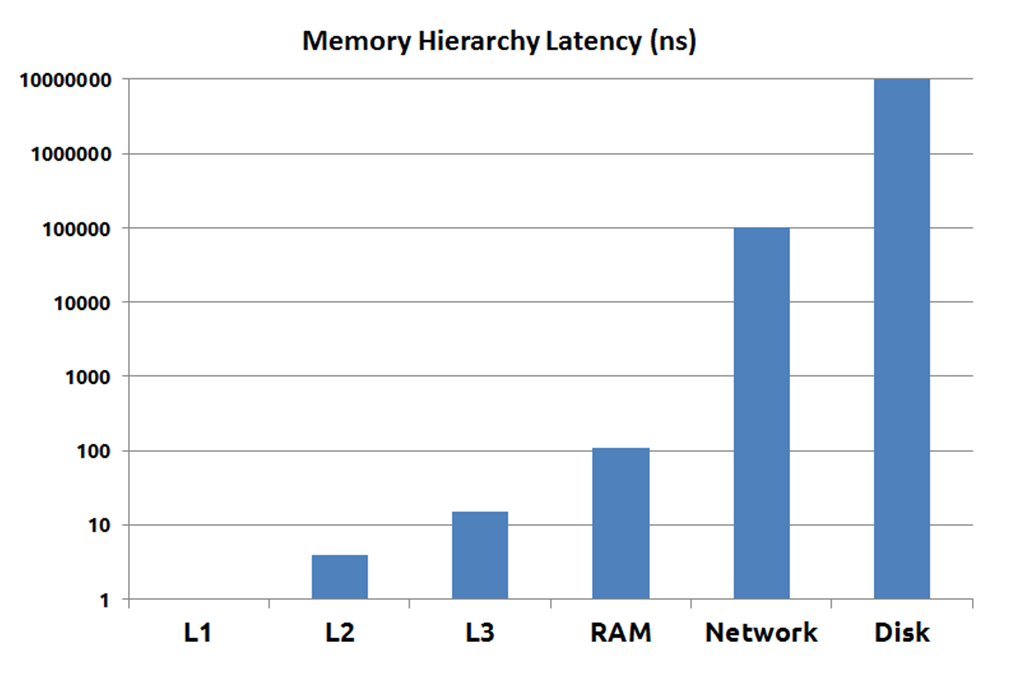
\includegraphics[width=70mm]{figures/memorylatency.png}
    \caption{Typical memory latencies in a modern commodity machine. Gigabit Ethernet latency included for comparison.}
    \label{fig:memlatency}
\end{figure}

Because of this fact, there is a lot more to parallel rendering than initially
meets the eye. Graphics may indeed by highly parallel, but its voracious
appetite for memory access is actively working \emph{against} its parallel
efficiency on current architectures.

This paper presents the architecture of FlexRender, a ray tracer designed for
rendering huge scenes with high geometric complexity on commodity hardware. We
specifically target commodity hardware because it currently has an excellent
cost to performance ratio, but still typically lacks enough memory to fit large
scenes entirely in RAM. Current strategies for parallelizing a renderer across
a cluster of commodity machines are limited to having each worker compute a
separate ``slices'' of the image (or frames of an animation), but do nothing to
manage the cost associated with large scene assets that do not fit into main
memory.

Thus, our work describes the following core contributions:

\begin{enumerate}
    \item A system for ray tracing which uses the pooled memory of a cluster of
        commodity machines to keep the entire scene in-core.
    \item A method for passing ray messages between workers in the cluster with
        enough state to never require a reply message.
    \item An extension to a stackless BVH traversal algorithm \cite{hapala:2011}
        that makes it possible to suspend traversal at one worker and resume it
        at another.
    \item A discussion of the concepts involved and an analysis of the resulting
        implementation.
\end{enumerate}

In particular, we show that FlexRender can achieve speedups that are around an
order of magnitude better than the traditional parallelization approach for
commodity machines, and can naturally self-regulate the cluster of workers to
keep the memory overhead due to message queuing around 1\% of each worker's
main memory.

\section{Background}
\label{background}

The FlexRender architecture builds on four fundamental building blocks:
Radiometry, ray tracing \cite{appel:1968} and \cite{whitted:1980}, bounding
volume hierarchies, and Morton coding.

\subsection{Radiometry and Ray Tracing}
\label{radiometryraytracing}

For a complete treatment of radiometry in the context of rendering algorithms
and ray tracing in general, we refer the reader to
\emph{Physically Based Rendering} \cite{pbrt}. For the purposes of FlexRender,
we note the following observations of the radiometry model of light:

\begin{description}
    \item[Light behaves linearly.] The combined effect of two rays of light
        in a scene is the same as the sum of their independent effects on the
        scene.
    \item[Energy is conserved.] When a ray reflects off of a surface, it can
        never do so with more energy than it started with.
\end{description}

FlexRender exploits these observations in the following ways:

\begin{description}
    \item[The location of computation does not matter.] If the scene is
        distributed across many machines, it makes no difference which machine
        computes the effect of a ray. The sum of all computations will be the
        same as if all the work was performed on a single machine.
    \item[Transmittance models energy conservation.] If we store the amount of
        energy traveling along a ray (the \emph{transmittance}) with the ray
        itself, we need not know anything about the preceding rays or state
        that brought this ray into existence. We can compute its contribution
        to the scene independently and ensure that linearity and energy
        conservation are both respected.
\end{description}

\subsection{Bounding Volume Hierarchies}
\label{bvhs}

Bounding volume hierarchies, or BVHs, are an application of binary search to 3D
space. BVHs are trees where each node is defined by a bounding volume, such as
a box or a sphere, that describes the extents of some region of space. All of
the primitives in the scene that are within that region are child nodes in the
tree.

The traversal algorithm of a BVH is naturally recursive, but recursive
implementations keep their state on the call stack. In FlexRender, we may need
to suspend the traversal on one machine and resume it on another, so we need
all of the traversal state explicitly exposed. Refactoring it as an iterative
traversal explicitly exposes the state for capturing, but unfortunately it still
requires a traversal stack of child nodes that must be visited on the way back
up the tree. In FlexRender, rays carry all necessary state along with them,
and this approach would require the entire stack to be included as ray state.

However, a stackless traversal method is described in
\emph{Efficient Stack-less BVH Traversal for Ray Tracing} \cite{hapala:2011}.
The key insight is that if parent links are stored in the tree, the same
traversal can be achieved using a three-state automaton describing the direction
you came from when you reached the current node (i.e. from the \emph{parent},
from the \emph{sibling}, or from the \emph{child}). They show that their
traversal algorithm produces identical tree walks and never retests nodes that
have already been tested.

FlexRender leverages this traversal algorithm due it its low state storage
requirements. Each ray only needs to know the index of the current node it is
traversing and the state of the traversal automaton. Our extensions to support
suspending traversal and resuming it on another machine are described in detail
in Section \ref{traversal}.

\subsection{Morton Coding and the Z-Order Curve}
\label{mortoncoding}

Morton coding is a method for mapping coordinates in multidimensional space to
a single dimension. In particular, walking the multidimensional space with a
Morton coding produces a space-filling Z-order curve.

\begin{figure}[h!]
    \centering
    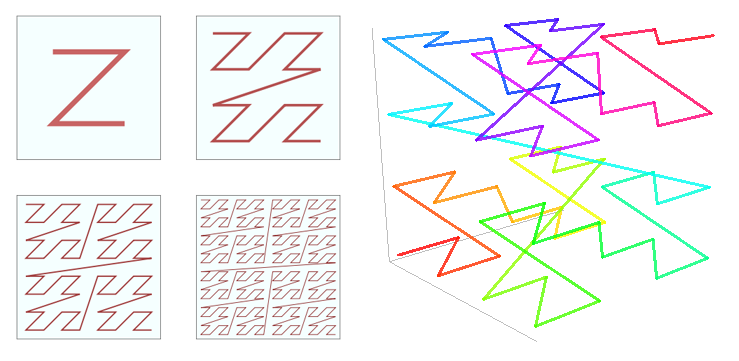
\includegraphics[width=70mm]{figures/zorder.png}
    \caption{Examples of two dimensional and three dimensional Z-order curves. Credit: ``David Eppstein'' and ``Robert Dickau'' (Creative Commons License)}
    \label{fig:zorder}
\end{figure}

More concretely, FlexRender needs a way to distribute a large scene to all the
machines in the cluster in a spatially coherent way. If the geometry on each
machine consists of a localized patch of the overall geometry, it allows us to
minimize communication between the machines, and thus, only pay the network cost
when we absolutely need to.

Because the Morton coding produces a spatially coherent traversal of 3D space,
dividing up the 1D Morton code address space among all the machines participating
in the render gives a reasonable assurance of spatial locality for the geometry
sent to each machine.

The Morton coding is also simple to implement. For example, say that we wish to
map a point $P$ in a region of 3D space (defined by its bounding extents
$min$ and $max$) to a Morton-coded 64-bit integer. Discretizing each axis evenly
allows for 21 bits per axis, yielding a 63-bit address space (and one unused bit
in the integer). We compute the Morton code by calculating the 21-bit
discretized component of $P$ along each axis, then shifting the components from
each axis into the 64-bit integer one bit at a time in a round robin fashion, from the
most-significant to least-significant bit.

\section{Related Work}
\label{relatedwork}

\subsection{Large Geometry}
\label{largegeometry}

A variety of computer graphics algorithms are designed to handle large-scale
geometry. Displacement maps \cite{krishnamurthy:1996} and normal maps using
texture data \cite{cohen:1998} and \cite{cignoni:1998} are commonly used,
especially in real-time applications. However, normal mapping displays visual
artifacts, particularly around the edges of the mesh (where it is clearly
apparent the surface is not high detail) or in areas where the texture is
scrunched or stretched. Similarly, level of detail is commonly used to replace
high resolution meshes with lower resolution versions when they are far enough
away from the viewer \cite{clark:1976}. However, it requires the creation of
multiple resolution meshes and algorithms to smoothly handle resolution changes.

Recent research has acknowledged that rendering data simply will not fit into
main memory any more, and has focused on techniques for efficiently using main
memory as a cache. In 2011, \cite{tabellion:2011} presented a technique for
dealing with huge point clouds used in point-based global illumination. They
showed that their method can process 88 GB of point cloud data with a cache of
just 2 GB, and can render 6.8 GB of point cloud data with cache hit rates of
over 99\%. One year earlier, \cite{pantaleoni:2010} showed that the software
they developed for Avatar was also very efficient at dealing with out-of-core
data. They generated directional occlusion data using ray tracing, which was then
compressed into spherical harmonics. The spherical harmonics were used at render
time (they did not directly ray trace the scenes during rendering). They used
hierarchical BVHs with a single ``top-level'' tree, which FlexRender also does.
However, they used it for chunking the scene into manageable units of work that
could be loaded and unloaded from main memory quickly.

\subsection{Parallel Rendering}
\label{parallelbg}

The most similar research to FlexRender is Kilauea \cite{kato:2002}, a massively
parallel networked ray tracer developed at Square USA in 2002. Similarly to our
work, it uses worker machines connected on a network to keep the entire scene
geometry in core. However, there are three main differences in our approach.

\begin{enumerate}
    \item \textbf{Geometry Distribution.}
        Kilauea randomly distributes geometry to its workers, then casts
        intersection rays through all workers simultaneously. The closest
        intersection is resolved from each worker's best candidate with a
        depth test. FlexRender distributes geometry such that workers ``own''
        a spatially local region, and passes rays between workers as they move
        through those regions.

    \item \textbf{Shading.}
        Kilauea suspends the execution of shaders for bounced rays, and resumes
        them when the rays come back through the system. It stores rays in a
        priority queue, sorted by termination likelihood. FlexRender maintains
        a similar priority queue, but carries source pixel and transmittance
        information along with each ray, making the suspension of shaders (and
        the associated overhead) unnecessary.

    \item \textbf{Latency Sensitivity.}
        Kilauea needs intersection results from every worker before proceeding
        with depth testing and shading, making the pipeline latency-sensitive.
        FlexRender computations are never waiting on results from another worker,
        so rendering clusters of hetergeneous machines (for example, CPU/GPU
        hybrid clusters) are not performance bottlenecks.
\end{enumerate}

Using GPGPU techniques, \cite{garanzha:2011:ray}, presented a
method for ray tracing large scenes that are out-of-core on the GPU. Parts of
their architecture are similar to FlexRender on a single-device scale,
specifically their use of heirarchical BVHs and ray queues to handle rays cast
from shaders. However, the global ray queue is fairly memory intensive,
potentially storing up to 32 million rays.

Leveraging MapReduce \cite{dean:2004}, \cite{northam:2011} presented an
implementation of a ray tracer, but noted that sending large amounts of scene
data to workers significantly slowed down processing. Their solution was to
break the scene into small chunks and resolve the intersection tests in the
reduce step. Unfortunately, this does a lot of unnecessary work, because many
non-winning intersections are computed that would have been pruned in a typical
BVH traversal.

\section{FlexRender Architecture}
\label{architecture}

In general, rendering with FlexRender proceeds in the following way:

\begin{enumerate}
    \item Read in the scene data and define the maximum bounding extents of the
        entire scene. As data is read in, it is distributed to the workers using
        the Morton coding.
    \item Once the scene is distributed, workers build BVHs in parallel for
        their respective local region of the scene. When complete, they send
        their maximum bounding extents to the renderer.
    \item The renderer constructs a top-level BVH from each of the workers'
        bounds and sends this top-level BVH to all the workers.
    \item Workers create image buffers. All shading computed on a worker is
        written to its own buffer. 
    \item Workers cast primary rays from the camera and test for intersections.
        \begin{itemize}
            \item During intersection testing, rays may be forwarded over the
                network to another worker if they need to test geometry within
                the bounding extents of that worker.
            \item Once the nearest intersection is found, illumination ray
                messages are created and sent to workers that have lights.
                These workers send light rays back towards the point of
                intersection to test for occlusion.
            \item If the light rays reach the original intersection, the point
                is illuminated and the worker computes shading.
        \end{itemize}
    \item Once all rays have been accounted for, workers send their image
        buffers back to the renderer, which composites them together into a
        final image.
\end{enumerate}

In the next few sections, we will examine each part of this process in greater
detail.

\subsection{Workers and the Renderer}
\label{workers}

There are two potential roles a machine can play during the rendering process.

\begin{description}
    \item[Worker] These machines receive a region of the scene and act as ray
        processors, finding intersections computing shading. They produce an
        image that is a component of the final render. There may be an
        arbitrary number of workers participating.
    \item[Renderer] This machine distributes scene data to the workers. Once
        rendering begins it monitors the status of the workers and halts any
        potential runaway situations (see Section \ref{primaryrays}). When the
        renderer decides the process is complete, it requests the image
        components from each worker and merges them into the final image.
        There is only a single renderer in any given cluster.
\end{description}

The network architecture is client/server connected in a star topology. Each
worker exposes a server which processes messages and holds client connections
open to every other worker for passing messages around the cluster. The renderer
also holds a client connection to every worker for sending configuration data,
preparing the cluster for rendering (described in Section \ref{prep}), and
monitoring render progress (described in Section \ref{completion}).

The current implementation does not include any provisions for fault tolerance.
However, there is no architectural restriction preventing such measures. For
topics involving the design of robust and resilient clusters, we refer the
reader to the distributed systems literature.

The graphics machinery is fairly straightforward. A \emph{scene} consists of a
collection of \emph{meshes}, which are stored as indexed face sets of vertices
and faces. Each mesh is a assigned a \emph{material}, which consists of a
\emph{shader} and potentially a set of bindings from \emph{textures} to names
in the shader. A \emph{shader} is a small program that computes the lighting on
the surface at a particular point.

\subsection{Fat Rays}
\label{fatrays}

The core message type in FlexRender is the \emph{fat ray}. They are so named
because they carry additional state information along with their geometric
definition of an origin and a direction. Their counterparts, \emph{slim rays},
consist of only the geometric components.

Specifically, a fat ray contains the following data:

\begin{itemize}
    \item The \textbf{type of ray} this is. See Section \ref{process}.
    \item The \textbf{source pixel} that this ray contributes to.
    \item The \textbf{bounce count}, or number of times this ray has reflected
        off a surface (to prevent infinite loops).
    \item The \textbf{origin} and \textbf{direction} of the ray.
    \item The ray's \textbf{transmittance}, (related to the amount of its final
        pixel contribution).
    \item The \textbf{emission} from a light source carried along the ray, if
        any. See Section \ref{illumination}.
    \item The \textbf{target intersection point} of the ray, if any. See
        Section \ref{illumination}.
    \item The \textbf{traversal state} of the top-level BVH. See Section \ref{traversal}.
    \item The \textbf{hit record}, which contains the worker, mesh, and $t$
        value of the nearest intersection.
    \item The \textbf{current worker} this ray should be forwarded to over the
        network.
    \item The \textbf{number of workers touched} by the ray. (Not
        used for rendering, only analysis.)
    \item A \textbf{next pointer} for locally queuing rays. Obviously invalid
        over the network. See Section \ref{queues}.
\end{itemize}

In total, the size of a fat ray is 128 bytes.

\subsection{Render Preparation}
\label{prep}

First, the renderer ensures that all the workers agree on basic rendering
parameters, such as the minimum and maximum extents of the scene, which is used
for driving Morton coding discretization along each axis. Once this data has
been synchronized with all workers, each worker establishes client connections
with every other worker that remain open for the duration of the render.

The renderer then divides up the 63-bit Morton code address space evenly by the
number of workers participating and assigns ranges of the address space (which
translate into regions of 3D space) to each worker. At this point the renderer
begins reading in scene data and takes the following actions with each mesh:

\begin{enumerate}
    \item Compute the centroid of the mesh by averaging its vertices.
    \item Compute the Morton code of the mesh centroid. The range this falls in
        determines which worker the mesh will be sent to.
    \item Ensure that any asset dependencies (such as materials, shaders, and
        textures) for this mesh are present on the designated worker.
    \item Send the mesh data to the designated worker.
    \item Delete the mesh data from renderer memory.
\end{enumerate}

Although the current implementation reads scene data in at the renderer
and distributes it over the network, there is no inherent reason why it needs
to do so. For example, if all workers have access to shared network storage,
the renderer could simply instruct each worker to load a particular mesh itself,
reducing load time.

\subsubsection{Parallel Construction of Bounding Volume Hierarchies}
\label{parallelbvh}

First, workers construct a BVH for each mesh they have for accelerating spatial
queries against the mesh. While building each BVH, the worker tracks bounding
extents of each mesh.

Next, workers build a root BVH for the entire region owned by the worker with
the mesh extents as its leaf nodes. When testing for intersections locally, a
worker first tests against this root BVH to determine candidate meshes, then
traverses each mesh's individual BVH to compute absolute intersections. After
construction of this root BVH, the root node's bounding extents describe the
spatial extent of all geometry owned by the worker.

Once construction of all local BVHs is complete, workers send their root
bounding extents to the renderer. The renderer then constructs a final top-level
BVH with worker extents as its leaf nodes. This top-level BVH is then distributed
to all workers. This is a quick and lightweight process, since the number of nodes
is only $2n - 1$, where $n$ is the number of workers. This top-level BVH guides
where rays are sent over the network in Section \ref{traversal}.

\subsection{Ray Processing}
\label{process}

Workers are essentially just multithreaded ray processors. Once rendering begins,
they continually pop rays from the ray queue, schedule them onto the thread pool,
and process them when the thread is run. This processing step consists of
testing for intersection, potentially forwarding the ray to another worker,
or computing shading values if the ray terminates.

There are three different types of rays:

\begin{itemize}
    \item \textbf{Intersection rays} identify points in space at which we would
        like to compute shading.
    \item \textbf{Illumination ray messages} are copies of intersection rays that
        have terminated. They are sent to workers who have emissive geometry.
        See Section \ref{illumination}.
    \item \textbf{Light rays} are Monte Carlo samples that contribute direct
        illumination to a point being shaded. See Section \ref{illumination}.
\end{itemize}

\begin{figure}[h!]
    \centering
    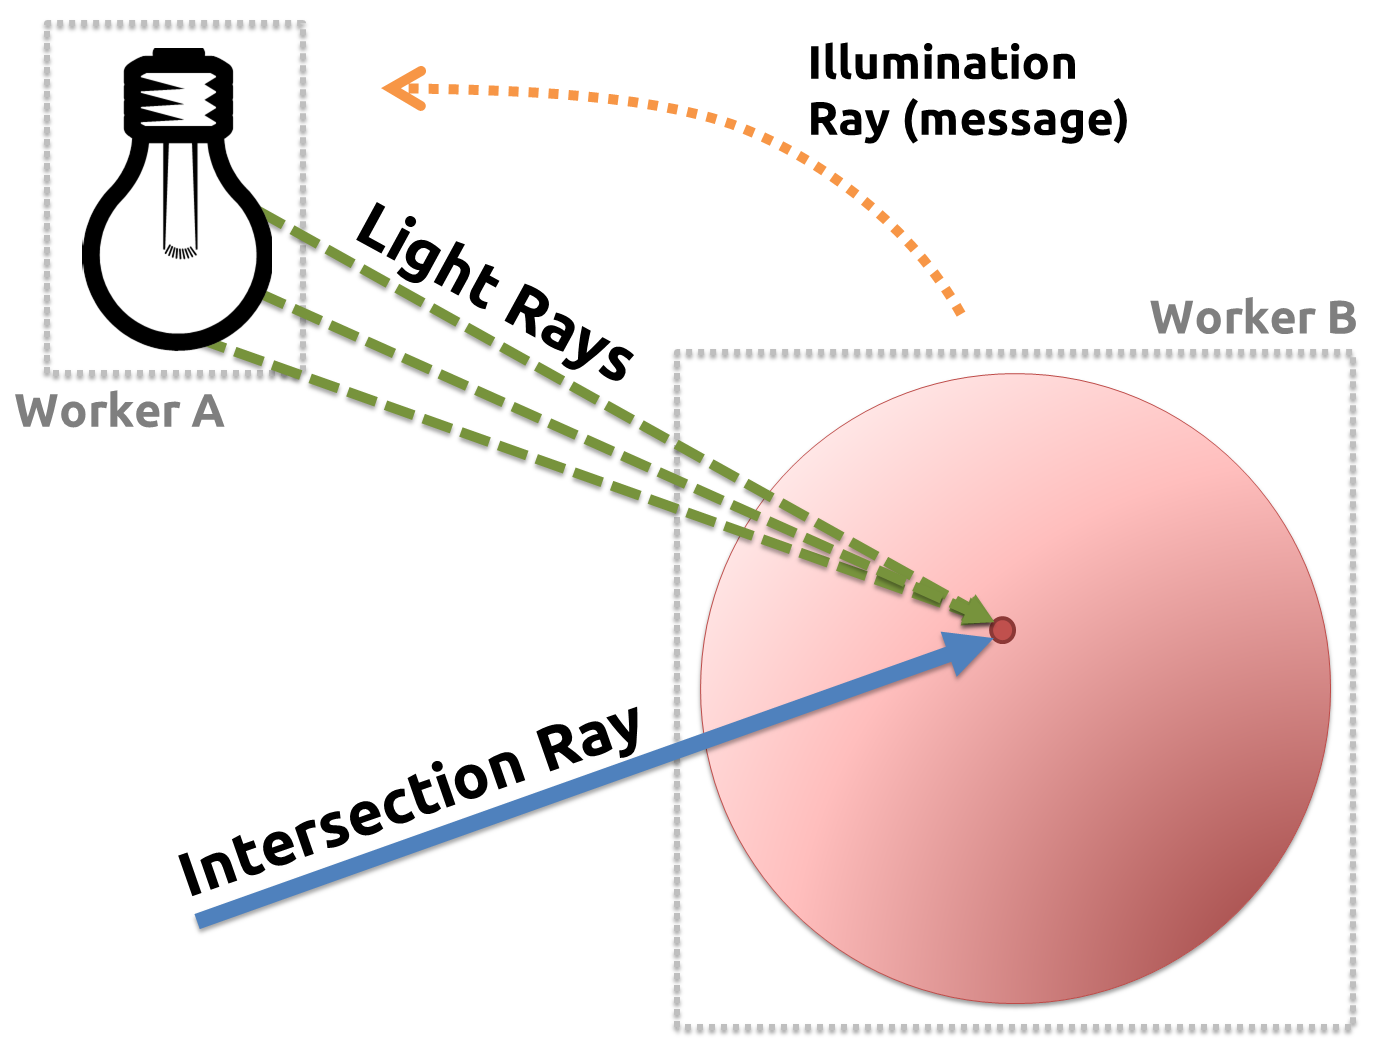
\includegraphics[width=60mm]{figures/raytypes.png}
    \caption{The three different ray types and their interactions.}
    \label{fig:raytypes}
\end{figure}

An important point is the sequence of their lifetimes. The order is as follows:

\begin{enumerate}
    \item An intersection ray is cast into the scene.
    \item When that intersection ray terminates at a point in space, it dies and
        spawns an illumination ray message sent to each worker with emissive
        geometry.
    \item When those illumination ray messages are delivered, they die and spawn
        light rays cast toward the original intersection.
    \item When those light rays terminate, they die. If they terminate at the
        original intersection, the worker computes shading for it.
\end{enumerate}

It should be apparent that a single intersection ray can spawn many additional
rays. It should also be apparent that light rays are the most likely to terminate
without generating additional rays.

\subsubsection{Illumination}
\label{illumination}

There is no special ``light'' type, only meshes that are emissive, which is a
property set by the assigned material. Emissive meshes are known to inject
light into the scene through their shader. During scene loading, the renderer
maintains a list of workers that have been sent at least one emissive mesh and
sends the list to all workers before rendering begins.

Once intersection testing has identified a point has been for shading, we
must determine the visibility of light sources from that point. In a traditional
ray tracer, shadow rays are cast from the point of intersection to sample points
on the surface of the light to determine visibility. However, from the perspective
of the worker computing shading, it has no idea where the lights in the scene
are, or if there is any geometry occluding the light.

To solve this problem, FlexRender traces shadow rays (which we call \emph{light rays})
in the opposite direction. Instead of originating at the intersection point and
traveling in the direction of the light, they originate at the light and travel
in the direction of the intersection point. Area lights are supported through
Monte Carlo integration by creating multiple light rays with origins sampled
across the surface of the light.

If a light ray returns to the original intersection point after being
traced through the cluster, we know its path from the light was unoccluded.
This leverages the same method for tracing rays through a distributed BVH that
we use for testing intersections. (See Section \ref{traversal}.)

In summary, illuminating an intersection is done as follows:

\begin{enumerate}
    \item On the worker where an intersection was found, copy the ray data into
        an illumination ray message with the target set to the point of
        intersection.
    \item Send the illumination ray message to all emissive workers.
    \item When a worker receives an illumination ray message, generate sample
        points across the surface of all emissive meshes. Set these sample
        points as the origins for new light rays.
    \item Set the directions of all the light rays such that they are oriented
        in the direction of the target.
    \item Push each light ray into the ray queue and let the cluster process
        them as usual.
\end{enumerate}


\subsubsection {Ray Queues}
\label{queues}

Each worker has a ray queue, with the typical push and pop operations for adding
and removing rays from the queue. This queue internally is implemented as three
separate queues, where rays are separated by type. It also contains information
about the scene camera, for generating new primary rays.

When a new ray arrives at a worker over the network, it is immediately pushed
into the queue. Internally, it is pushed into the queue matching its type
(intersection, illumination, or light).

When the worker pops a ray from the queue, we pull rays from the internal
queues in the following order:

\begin{enumerate}
   \item The \textbf{light queue}, since these are least likely to generate
      new rays.
   \item If the light queue is empty, we pop from the \textbf{illumination queue},
      since these will generate a limited number of new rays.
   \item If the illumination queue is empty, we pop from the
      \textbf{intersection queue}, since these can generate the most new rays.
   \item If all of the internal queues are empty, we use the camera to cast
      new primary rays into the scene (described in \ref{primaryrays}). This
      effectively generates new work.
\end{enumerate}

Organizing the processing order of rays as a priority queue based on ray type
is an essential step in minimizing the exponential explosion of work than can
occur if too many primary rays enter the system at a time. This helps reduce
memory usage required for queuing messages because new work is not generated
until the system is ready to handle it.

\subsubsection{Primary Ray Casting}
\label{primaryrays}

The workers in the cluster are each responsible for casting a portion of the
primary rays in the scene. The reasoning behind this is to give the cluster
the ability to regulate itself.

Consider the case where a worker has not received any work recently from other
workers in the cluster. For whatever reason (intersection tests, shading, etc.)
the other workers are too busy dealing with their own queues to send any work
in the direction of our lonely, rayless worker. By giving the worker control
over primary ray casting for a portion of the scene, we give workers the ability
to generate work when they have nothing to do.

However, consider the case where a worker contains mostly background
geometry. It will be receiving work from others infrequently because its size
in screen space is small, but yet it is in charge of casting primary rays for
a much larger slice of the image. In this case the worker may go on an
unfettered spree of primary ray casting, causing lots of grief for his fellow
workers since he is essentially generating work for others and little for
himself.

To prevent this ``runaway'' case from overburdening the ray queues, we require
that workers report statistics about their progress to the renderer every so
often (10 times per second in the current implementation). If the renderer
notices that a worker is getting significantly further ahead of the others in
primary ray casting, we temporarily disable primary ray casting on that worker
until the others catch up.

Because the other workers will not generate primary rays as long as they still
have other rays in their queues to process, the priority queuing, shared
ray casting responsibilities, and temporary pausing of primary ray generation at
runaway workers provides a simple means of self-regulating the cluster that
works remarkably well and minimizing the memory overhead for message queuing.
We will examine the overhead in detail in section \ref{results}.

\subsubsection{Distributed BVH Traversal}
\label{traversal}

To understand how distributed traversal of the top-level BVH works, consider
the following example traversal of this top-level tree with 5 workers (letters
A through E) participating in the render.

%\begin{figure}[H]
%    \centering
%    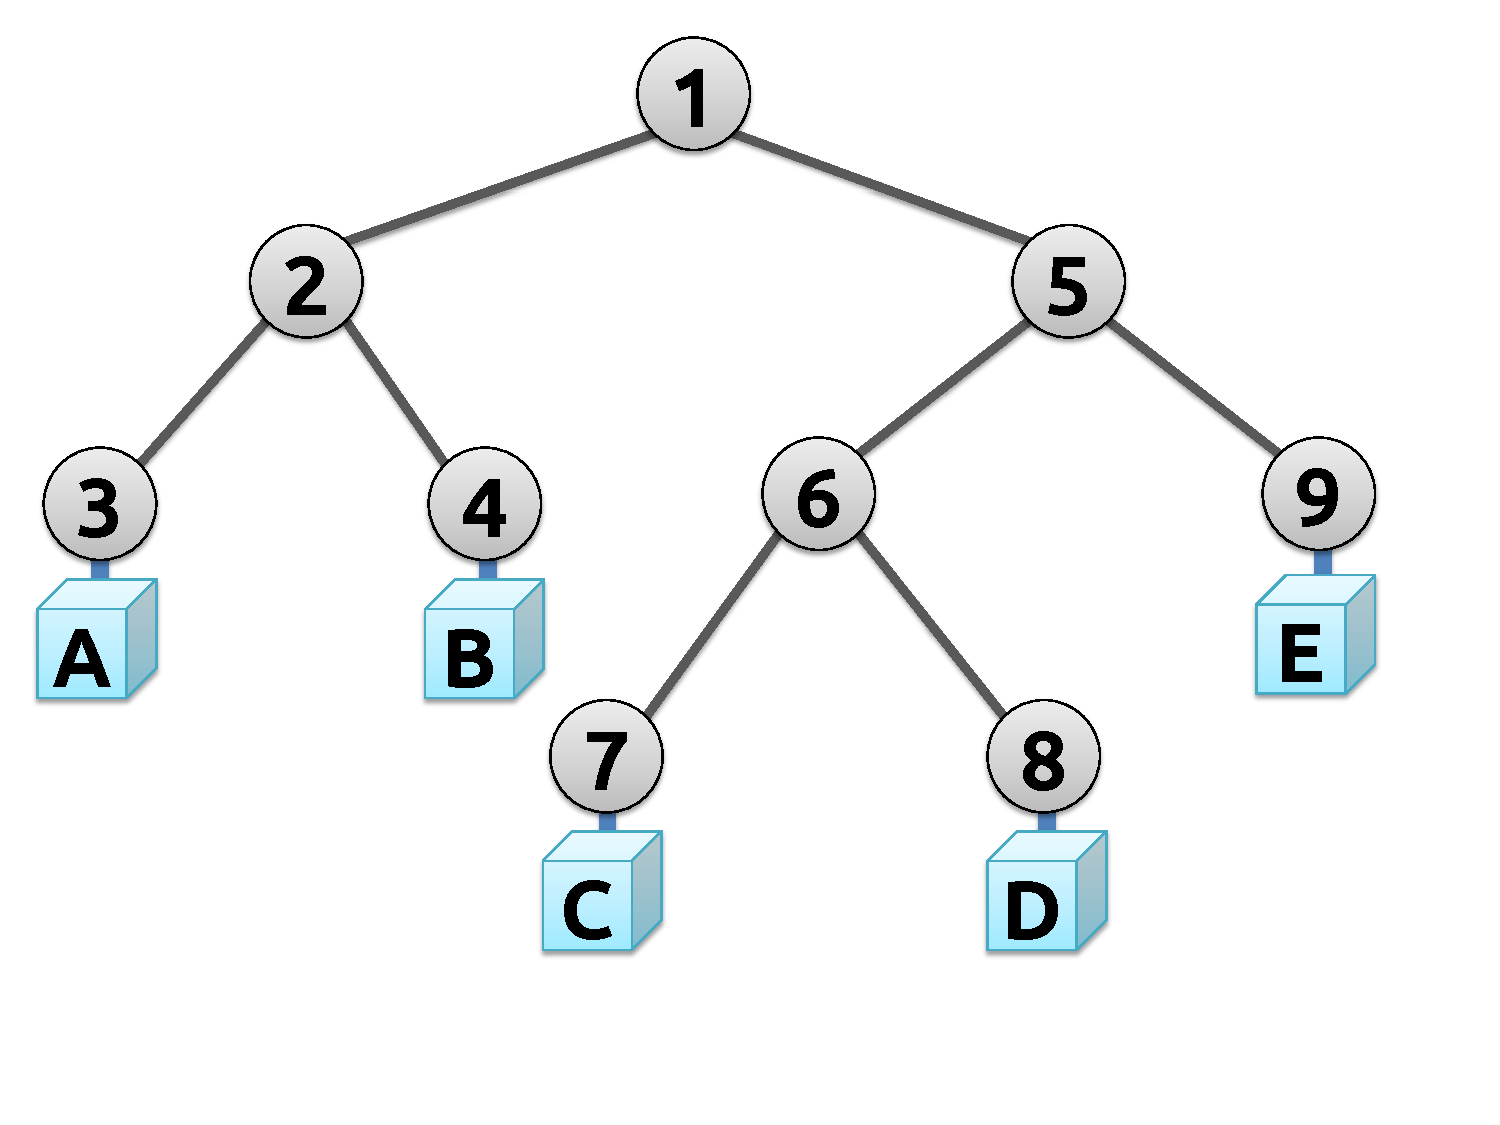
\includegraphics[width=80mm]{figures/traversal1.pdf}
%    \caption{Example top-level BVH with 5 workers.}
%    \label{fig:traversal1}
%\end{figure}

The worker who generates the ray begins traversing the tree by checking the ray
against the bounds of the left-hand child. If the ray fails the test, we move
to check its sibling, right-hand child.

\begin{figure}[h!]
    \centering
    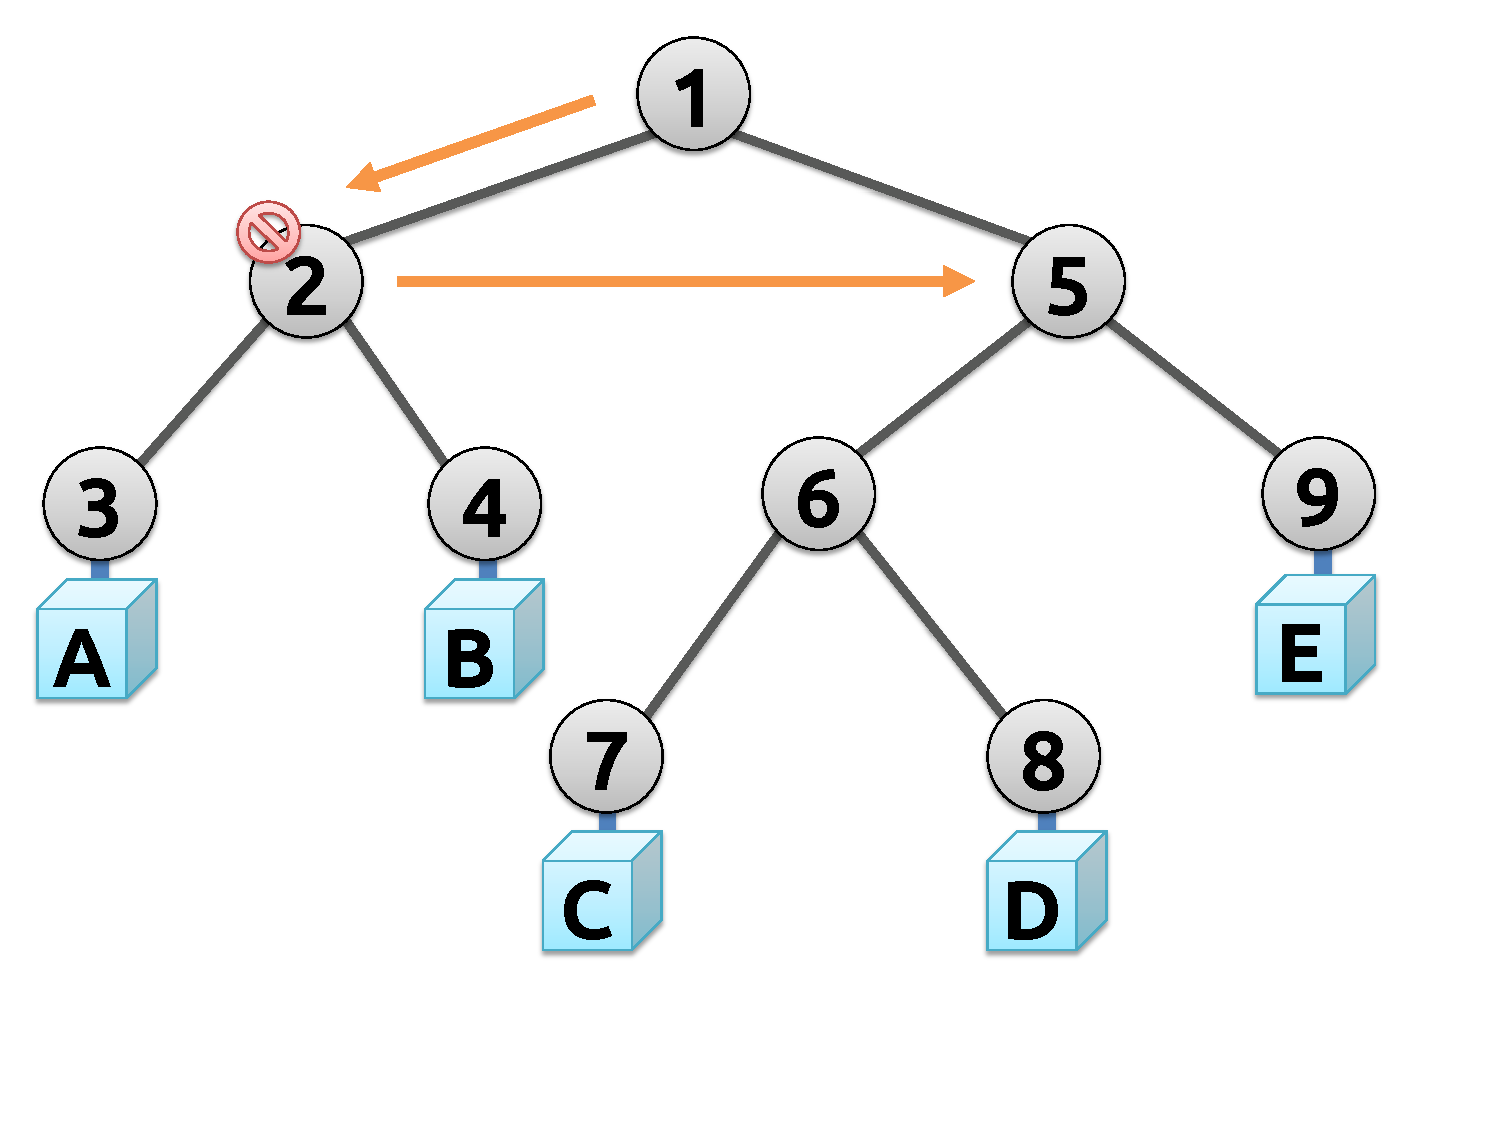
\includegraphics[width=60mm]{figures/traversal2.pdf}

    \caption{The ray fails its first test and moves to the sibling node.}
    \label{fig:traversal2}
\end{figure}

This test passes, so we continue down the tree to that node's left-hand child.
Let us assume this test also passes.

\begin{figure}[h!]
    \centering
    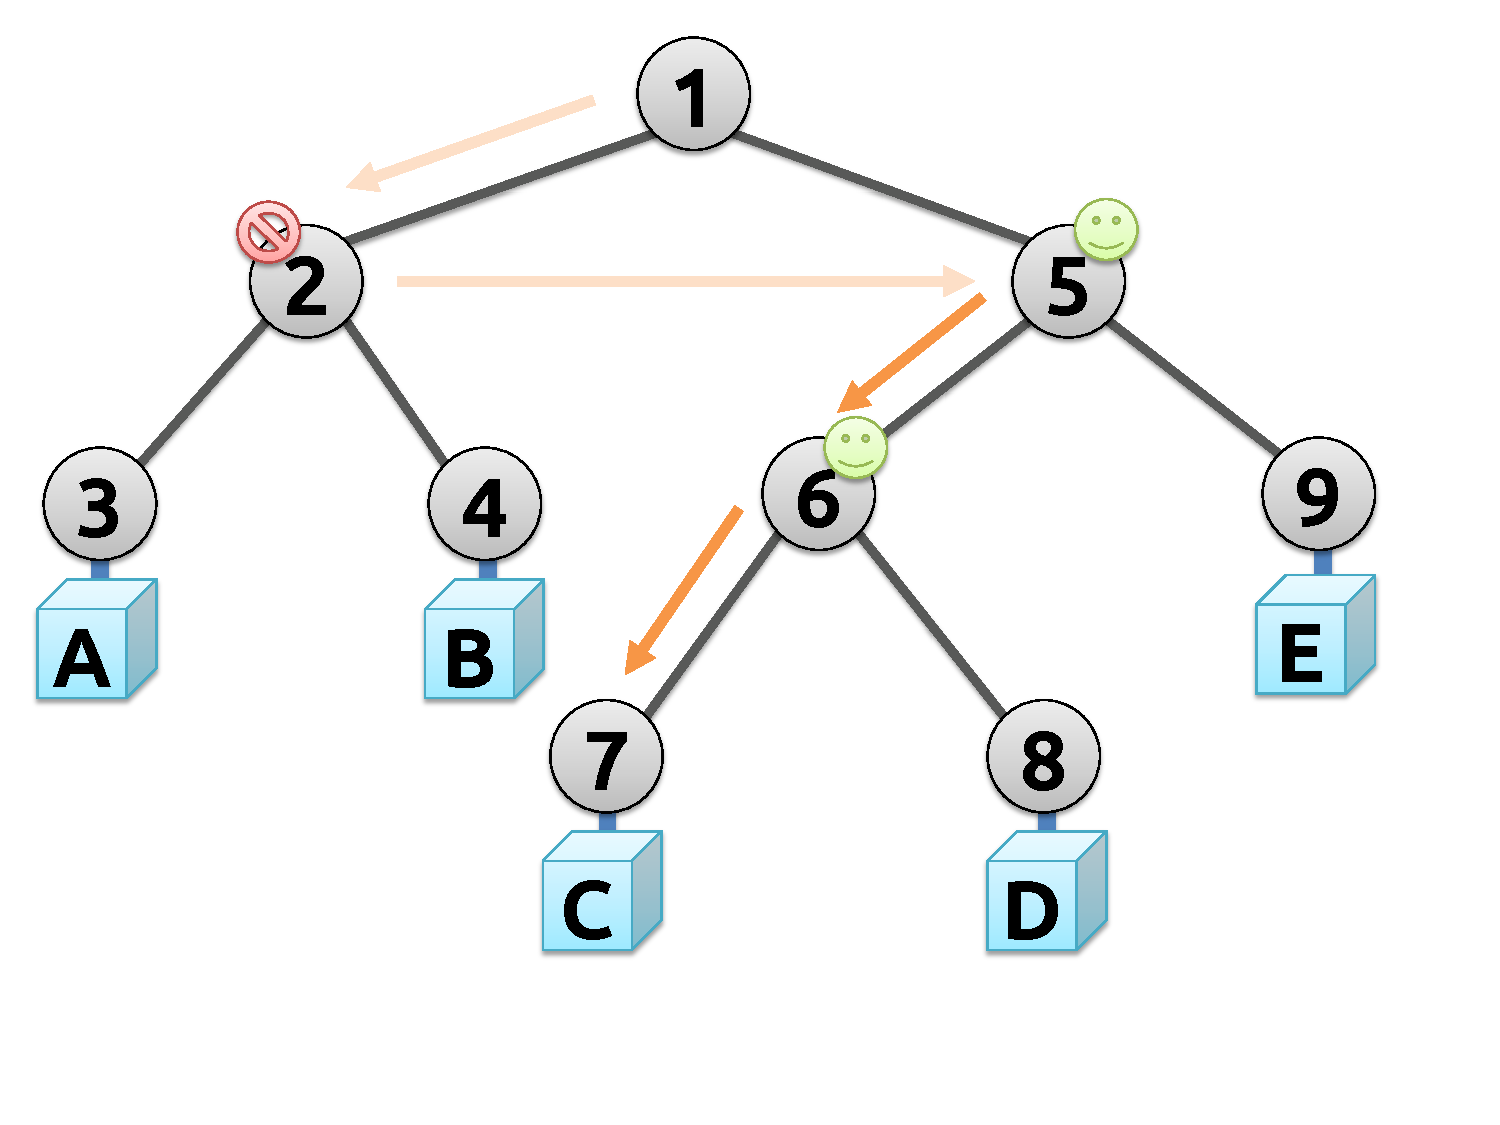
\includegraphics[width=60mm]{figures/traversal3.pdf}

    \caption{Traversal down the left-hand nodes continues as long as bounding tests pass.}
    \label{fig:traversal3}
\end{figure}

We test our first leaf node, and it passes. This indicates we must test the
geometry on the worker itself. This is where our primary modification to the
Hapala et al \cite{hapala:2011} algorithm occurs. Rather than continuing to
traverse the tree, we immediately jump out of the function the return the
traversal state. The traversal state consists of the index of the current
node, and the automaton defining where we came from (7 and \emph{from the parent}
respectively). We store this traversal state in the ray and pass it off to worker
C.

When worker C unpacks the ray and begins to process it, it notices that the
state of the traversal is not at the root of the tree, which means this is a
ray whose traversal was suspended. Because a suspended ray would never be sent
to a node for any other purpose than an intersection test, worker C immediately
tests for intersections against its geometry. For the purpose of this example,
let's say it hits nothing.

\begin{figure}[h!]
    \centering
    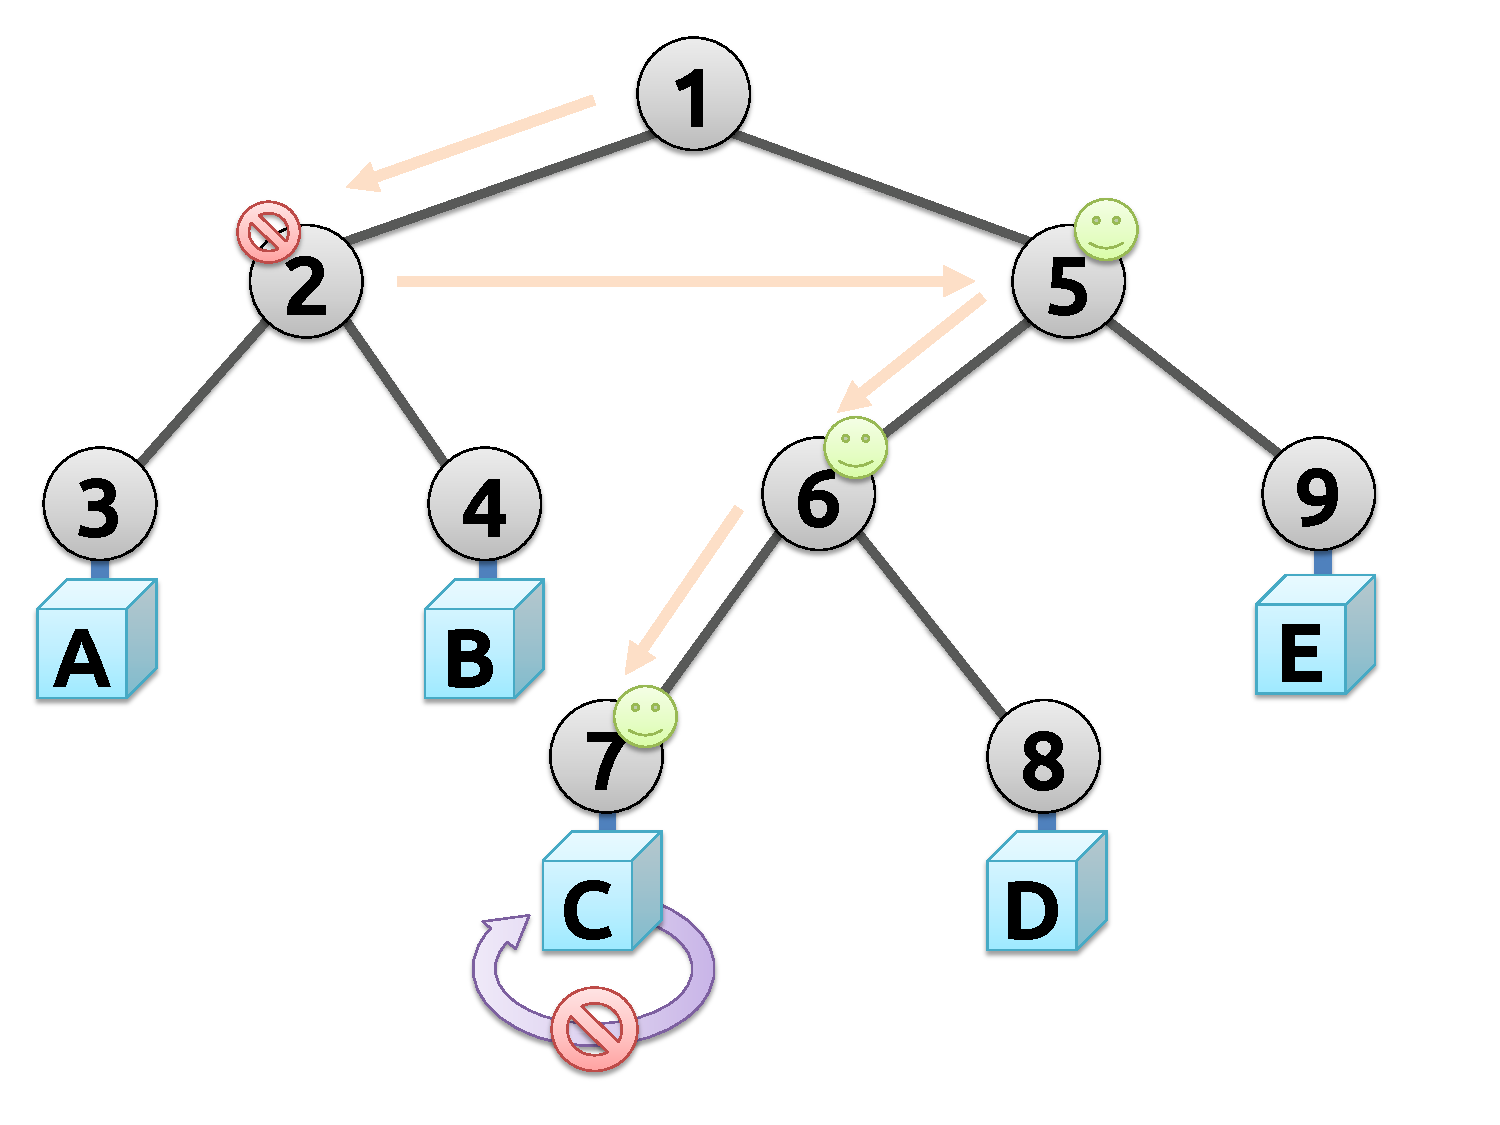
\includegraphics[width=60mm]{figures/traversal4.pdf}
    \caption{The ray is sent to worker C and tested against local geometry for intersections.}
    \label{fig:traversal4}
\end{figure}

The traversal state is then reinstated (node 7, \emph{from the parent}) and
worker C jumps immediately to where it left off, testing the bounds of C's
sibling, worker D. It hits the bounds, so again, we pack up the traversal
state (now node index 8 and \emph{from the sibling}) and ship off the ray to
worker D.

\begin{figure}[h!]
    \centering
    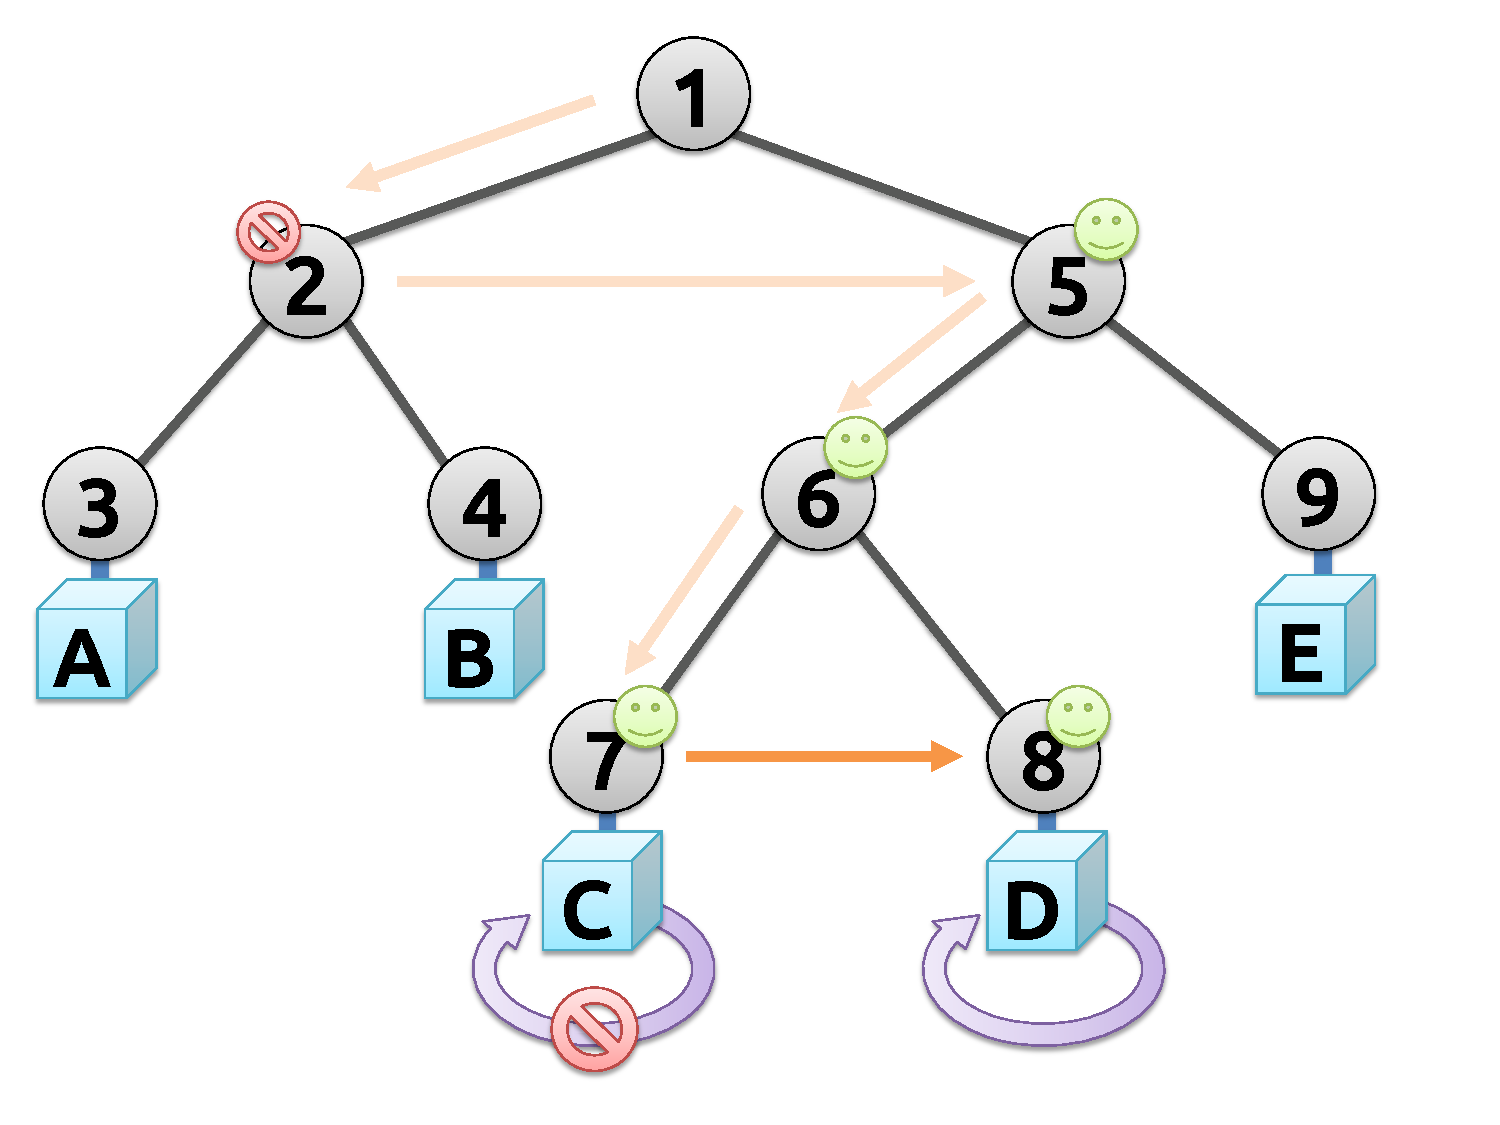
\includegraphics[width=60mm]{figures/traversal5.pdf}
    \caption{The ray is sent to worker D and again tested against local geometry for intersections.}
    \label{fig:traversal5}
\end{figure}

Worker D goes through the same process. Since the ray is suspended, it checks
its local geometry for intersections. Let's say it hits a mesh 42 at distance
of 10 units along the ray. This forms a hit record, which is stored inside the
ray (worker D, mesh 42, 10 units).

Again we reinstate the traversal state (node 8, \emph{from the sibling}) and
traverse back up to the parent (node 6). Since our state entering node 6 is
\emph{from the child}, we move next to node 9, another leaf node, and test
its bounds against the ray.

%\begin{figure}[H]
%    \centering
%    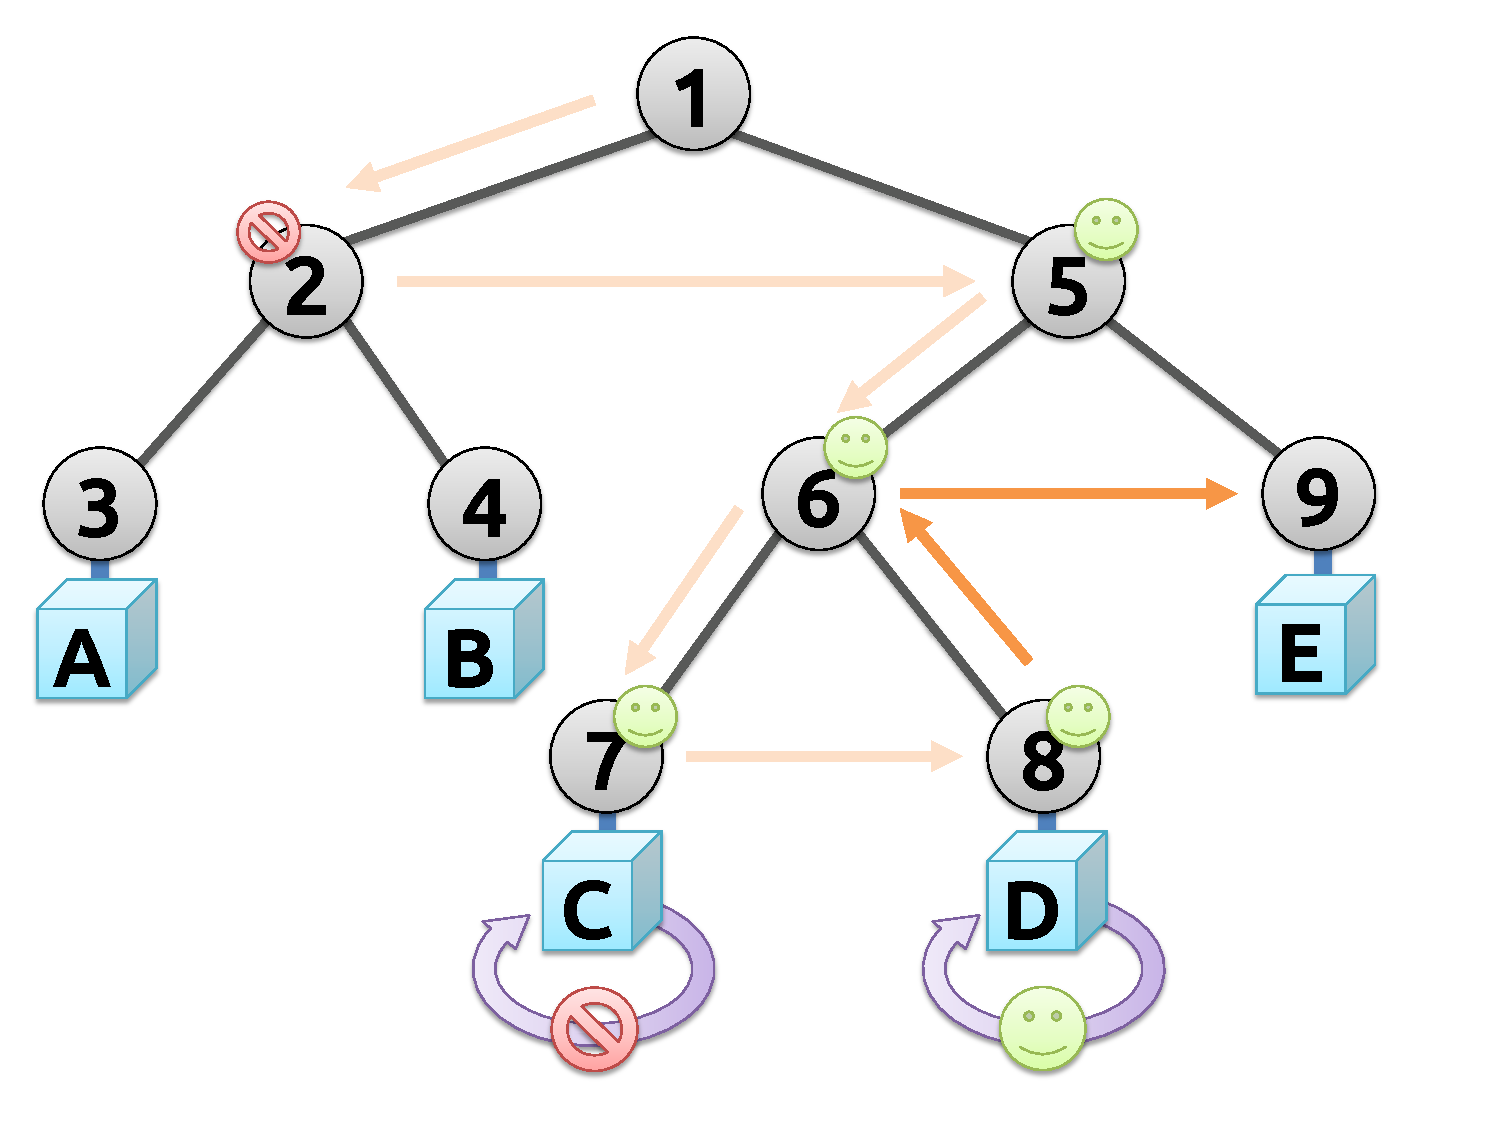
\includegraphics[width=80mm]{figures/traversal6.pdf}
 %   \caption{With successful hit record in hand, traversal continues back up the tree.}
  %  \label{fig:traversal6}
%\end{figure}

Let's say this also passes. However, the ray intersects the bounds at a distance
of 20 units along the ray. The closest an intersection on worker E could
possibly occur is further away, so there is no point to sending the ray to
worker E. Thus, we do not send the ray to worker E and continue to traverse up
the tree until we reach the root again.

%\begin{figure}[H]
%    \centering
%    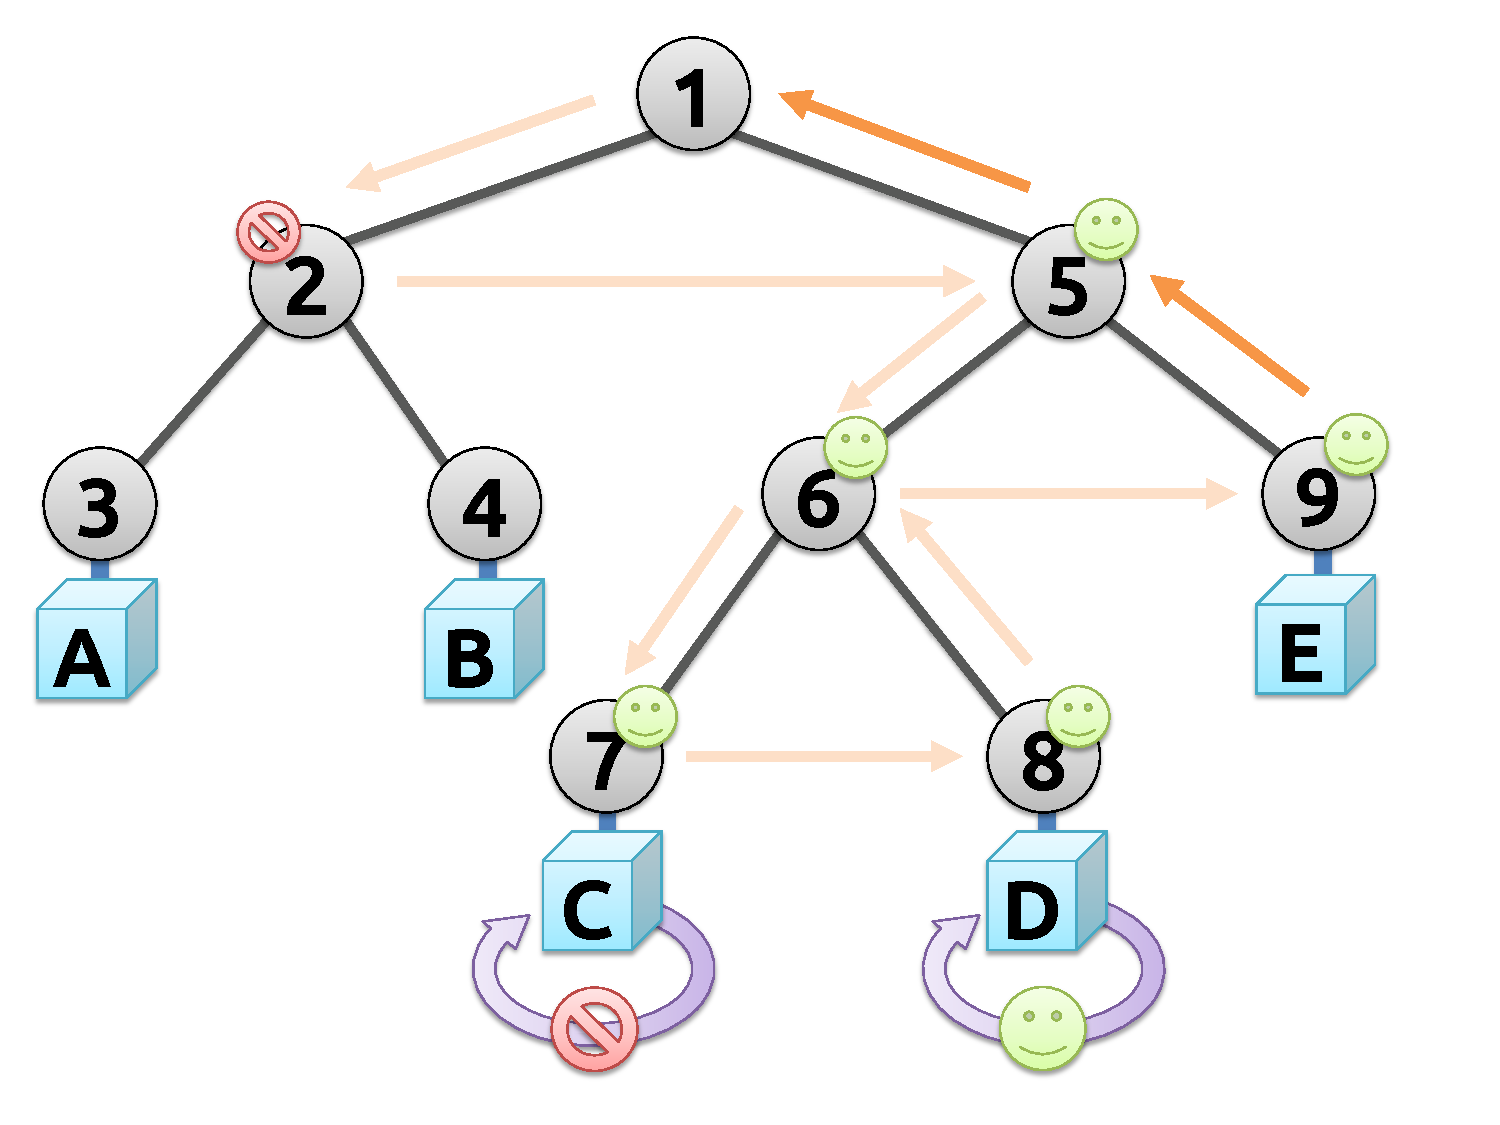
\includegraphics[width=80mm]{figures/traversal7.pdf}

%    \caption{Worker E's bounding test passed, but was further away than the hit record. We arrive at the root and traversal is complete.}
%    \label{fig:traversal7}
%\end{figure}

Once we reach the root, we know the top-level traversal is complete. At this
point we only need to consult the ray's hit record to determine which mesh on
which worker yields the closest intersection.

In the best case, a ray is generated on, intersects only with, and is shaded on
a single worker. These rays never need to touch the network. In the worse case,
the ray potentially intersects with all nodes, so it must touch every node in
the tree before being sure of its intersection point.

In addition, there are two interesting corner cases to consider.

\begin{itemize}
    \item If the ray is generated on a node that it does not intersect until
        later in the traversal, it consumes one additional network hop at the
        very beginning of the traversal.
    \item If the ray completes its traversal on a worker different from that
        which had the closest intersection, it consumes one additional network hop
        at the end of the traversal to put the ray on the correct node for
        shading.
\end{itemize}

Thus, the worst case scenario actually touches $n + 2$ workers, where $n$ is the
number of workers in the cluster.

In section \ref{futurework}, we discuss possible optimizations that may eliminate
both of these corner cases. Additionally in section \ref{results}, we show that
in practice, the number of workers that each ray touches is less than or equal
to the predicted $O(log\;n)$ expansion of the binary tree for the majority
of rays in the scene.


\subsubsection{Shading}
\label{shading}

When a light ray arrives at a worker, we simply check that its point of
intersection is within some epsilon of the target. If it is, we consider the
light sample visible, look up the material, shader, and textures for the mesh,
and run the shader. The shader is responsible for writing its computed values
into the worker's image buffer.

The implementation of shaders in FlexRender is through extensions to the Lua
\cite{lua} programming language, using the LuaJIT \cite{luajit} implementation
for speed. A shader may do any (or none) of the following:

\begin{enumerate}
    \item Sample textures based on the name bindings assigned in the material
        definition.
    \item Compute a light value based on some implementation of a mathematical
        shading model (such as the Phong model) and local information at the
        point being shaded (such as the interpolated surface normal and texture
        coordinates).
    \item Accumulate computed light values into the primary RGB buffers, or
        any auxiliary named buffer.
    \item Cast additional rays into the scene.
\end{enumerate}

When new rays are cast into the scene from a shader, the results of that trace
are not immediately available. Instead, the trace pushes the new rays into the
queue for processing and the traversal and shading systems ensure that the
result of secondary and $n$-ary traced rays will be included in the final image.

In order for linearity and energy conservation to be respected, certain values
are inherited from the parent ray. In particular, the source pixel is inherited
(so the ray contributes to the correct pixel in the final image) and the
desired transmittance along the new ray is multiplied with the transmittance of
the parent ray (to ensure energy conservation is preserved).  Casting rays from the shader can be used to implement several common visual
effects:Alpha masking, Reflection, Refraction, Monte Carlo global illumination can all be acheived 
by casting new rays with the appropriate direction.


\subsection{Render Completion}
\label{completion}

In a traditional recursive ray tracer, determining when the render is complete
is a simple task. Once the last primary ray pops its final stack frame
the render is over. In FlexRender, however, no one worker (or the renderer, for
that matter) knows where the ``last ray'' is. To determine when a render is
complete,  the workers report general statistics
about their activities to the renderer at regular intervals (in our current
implementation, 10 times per second). In particular, the following four
statistics are useful for determining if the render has finished:

\begin{description}
   \item[Primary Ray Casting Progress] The amount of the worker's primary rays
      that have been cast into the scene.
   \item[Rays Produced] The number of rays created at the worker during this
      measurement interval. This includes new intersection rays cast from the
      camera or a shader, illumination ray messages created by terminating intersection
      rays, or light rays created by processing illumination ray messages.
   \item[Rays Killed] The number of rays finalized at the worker during this
      measurement interval. This includes intersection rays that terminated or
      did not hit anything, illumination ray messages that were destroyed after spawning
      light rays, or light rays whose final shading value was computed.
   \item[Rays Queued] The number of rays currently in this worker's ray queue.
\end{description}

In particular, if any worker has not finished casting its primary rays, we
know for certain the render is not complete. Secondly, if we observe that no
rays are produced, killed, or queued at any workers for some number of
consecutive measurement intervals, it is reasonable to assume that the render
has concluded. Our current implementation (which reports statistics 10 times per second)
waits until it sees 10 consecutive intervals of ``uninteresting'' activity on
the workers before declaring the render complete. We find this achieves a nice
balance between wanting to end the render as soon as it is legitimately
finished and risking concluding it too early.

\subsubsection{Image Synthesis}
\label{synthesis}

Once the render has been deemed ``complete'', the renderer requests the image
buffers from each worker. Because all rendering was computed by respecting
linearity, computing a pixel in the final output image is just a matter
of summing corresponding pixels in the worker buffers.

This can yield some interesting intermediate images. Each worker's buffer
represents the light in the final image that interacts in some way with the
geometry present on that worker. For direct light, this shows up as shaded samples where geometry was present
and black areas where it was not. For other effects such as reflections and
global illumination, it appears that the worker had access to the whole scene's
geometry all along, but this is just an optical illusion. Since the rays
carry with them the source pixel they contribute to (and this value is inherited
as new rays are spawned from the primary ray), a worker can end up contributing
to any pixel in the image as long as the light interacted in some way with the
geometry it controlled.

\begin{figure}[h!]
    \centering
    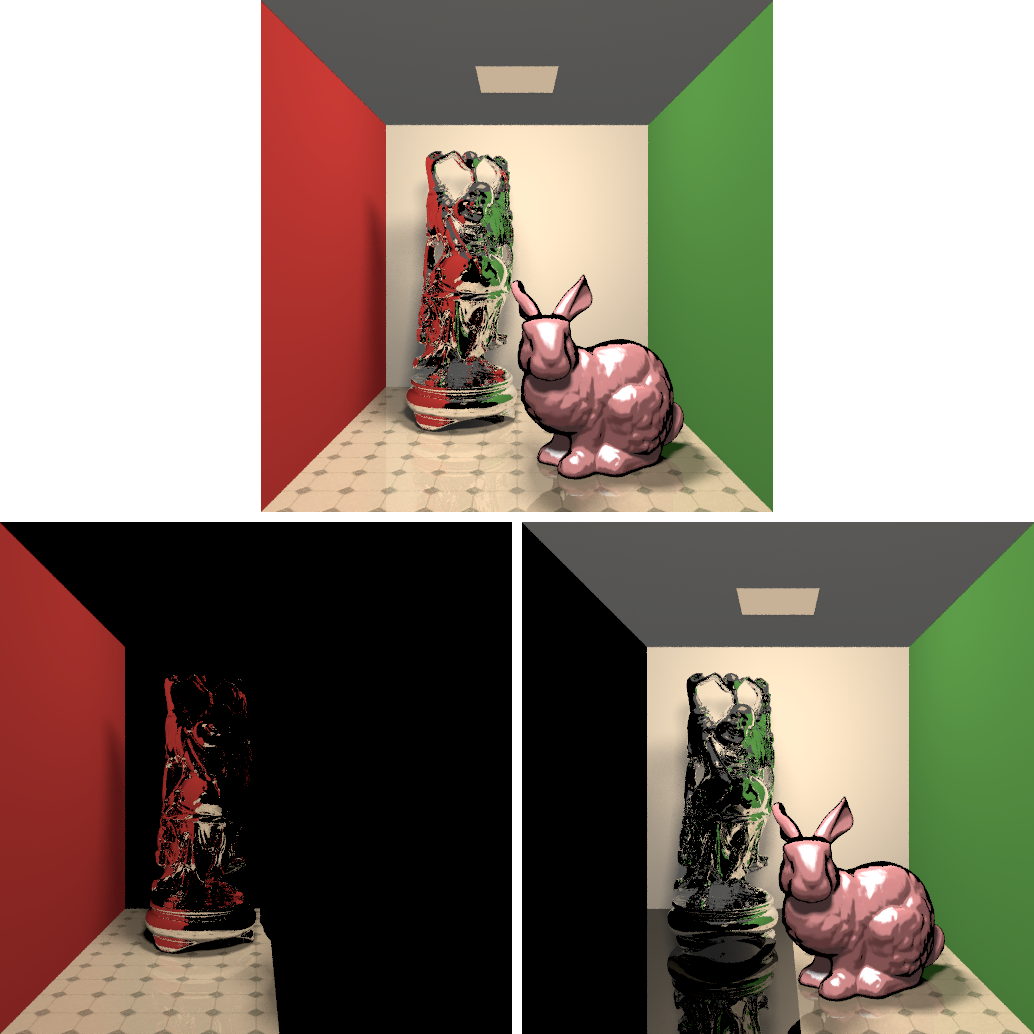
\includegraphics[width=80mm]{images/linearity.png}
    \caption{The left and right images show the geometry split between two workers. The composite image is in the center. Note how the Buddha reflects the left side geometry in the left image and the right side geometry in the right image. The actual Buddha mesh data was distributed to the worker on the left.}
    \label{fig:linearity}
\end{figure}

\section{Results}
\label{results}

For testing, we used 2-16 Dell T3500 workstations with dual-core Intel Xeon
W3503 CPUs clocked at 2.4 GHz. Each workstation had 4 GB of system RAM, a 4 GB
swap partition, and was running CentOS 6.  On the software side, FlexRender consists of around 14,000 lines of code. Of
that, 80\% is C++, 17\% is Lua (scene and
shader support libraries), and 3\% is Bash script used for building library
dependencies.  We leverage several popular open source libraries: \emph{LuaJIT}, \emph{libuv}, \emph{MsgPack}, \emph{GLM} and \emph{OpenEXR}.  We also made use of the \emph{pfstools} and \emph{pdiff} software packages
for tone mapping our output images and computing perceptual diffs respectively.

\subsection{Test Scene}
\label{toystore}

Our test scene, ``Toy Store'', has a geometric complexity of nearly 42 million
triangles. The room geometry is relatively simple, but the toys on the shelves are unique
(non-instanced) copies of the Stanford bunny, Buddha, and dragon models that
have been remeshed from their highest quality reconstructions down to 14,249
faces, 49,968 faces, and 34,972 faces respectively. There are 30 toys per
shelf and 42 shelves in the scene for a total of nearly 1,300 models. Approximately
one quarter of the models are rendered with a mirror shader. The others have
a standard Phong shader.  The scene consists of 1.09 GB of mesh data and 5 GB of BVH data once the
acceleration structures are built.  

A test  image was rendered at a resolution of 1024x768 with no subpixel antialiasing,
10 Monte Carlo samples per light (32 lights in the scene), and a recursion
depth limit of 3 bounces.  For discussing render time speedups, we will consider the specific case of 8
workers in the traditional configuration vs. 8 workers in the FlexRender
configuration. 

\paragraph{Traditional Method vs. FlexRender}

To compare FlexRender to current techniques, we considered a traditional method of rendering
such a large scene on 8 workers, which chopped up the image into several vertical
slices, with a different machine responsible for each slice. The slices are
then reassembled to form the final output image.

\begin{figure}[h!]
    \centering
    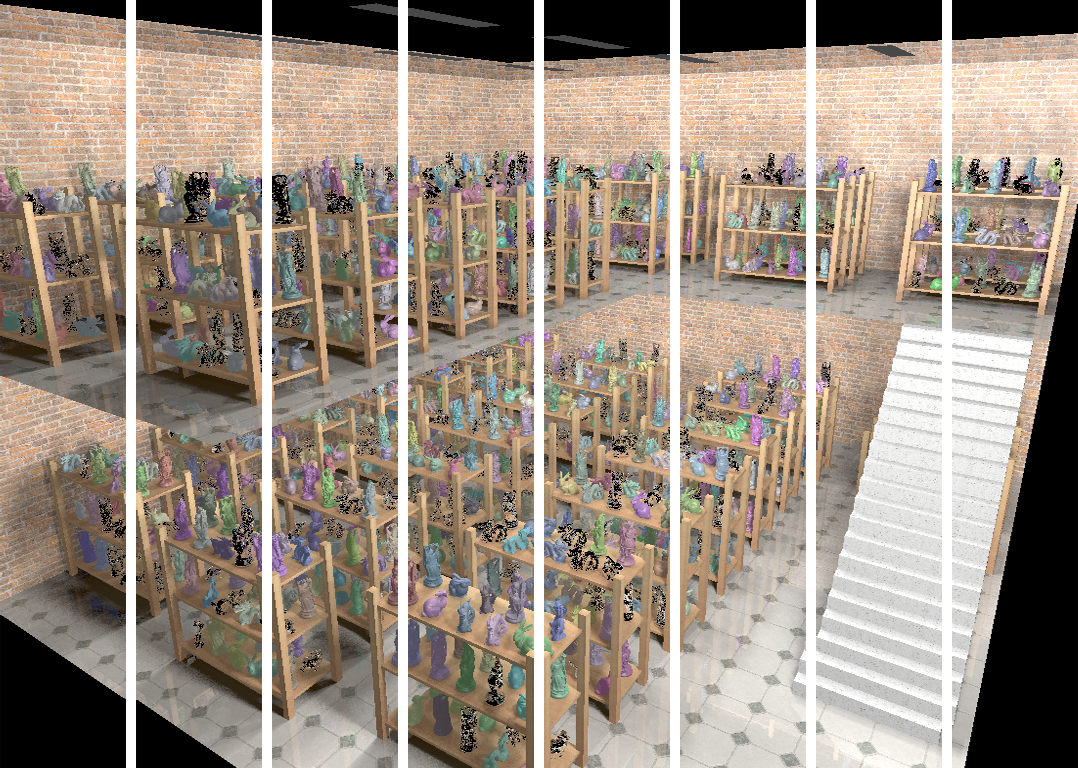
\includegraphics[width=80mm]{images/toystore-sliced.png}

    \caption{Slices of the Toy Store scene rendered with 8 machines in the traditional configuration used as a comparison to renders using FlexRender (composite result image shown in Figure~\ref{fig:sotoystore}).}
    \label{fig:toystoresliced}
\end{figure}

We report time for each machine to complete each phase of rendering (loading
the scene, building the BVH, and rendering its slice of the image) in the right side of Table
\ref{tb:traditionaltimes}. In particular, the total length of the render would
take 10,061 seconds (the slowest time), because the last slice is needed before
the final image can be reassembled.  We report average times for the traditional workers
compared to FlexRender for each of the 3 rendering phases in Table
\ref{tb:flexrendertimes} and show FlexRender's speedup over the average case.  We also report the total render time (all three phases combined), using this
time the slowest traditional worker. 

\begin{table}
\begin{center}
\begin{tabular}{|l||c|c|c||c|}
    \hline
    & load & BVH & render & \textbf{total}\\
    \hline
    \hline
  1 & 288 & 169 & 533 & 990\\
    \hline
    2 & 290 & 172 & 1119 & 1581 \\
    \hline
    3 & 290 & 167 & 1491 & 1948 \\
    \hline
   4 &  289 & 261 & 9511 & 10061 \\
    \hline
    5 & 295 & 174 & 1792 & 2261 \\
    \hline
    6 & 290 & 192 & 677 & 1159\\
    \hline
    7 & 287 & 167 & 1109 & 1561 \\
    \hline
    8 & 294 & 171 & 303 & 768 \\
    \hline
\end{tabular}
\caption{Timings for each phase of the algorithm  for each of the 8 workers. Times (in seconds) are given for individual workers to complete each phase using the traditional method:  loading, building a BVH, rendering and the total time of all three phases.}
\label{tb:traditionaltimes}
\end{center}
\end{table}

\begin{figure}[h!]
    \centering
    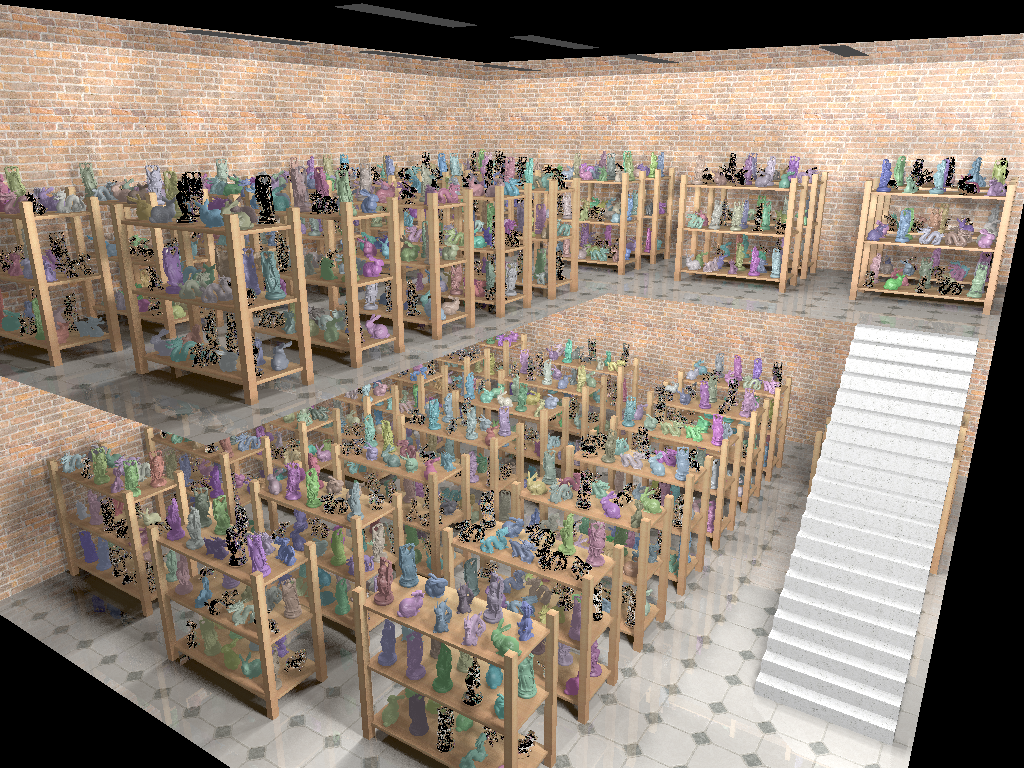
\includegraphics[width=80mm]{showoff/toystore.png}
    \caption{Toy Store scene that is comprised of nearly 1,300 models and 42 million triangles.}
    \label{fig:sotoystore}
\end{figure}


%Lastly, we also report the times and speedup excluding the loading and syncingphase. The reasoning behind this is that while FlexRender currently reads inscene assets at the renderer and distributes them across the network, there isno inherent reason why it needs to load the scene this way. Specifically,if each worker had access to a shared network storage volume with the sceneassets on it, the renderer could simply issue commands to each workerinstructing it to load a particular asset from the network storage.

\begin{table}
\begin{center}
\begin{tabular}{|l||c|c|c|}
    \hline
    & Traditional & FlexRender & Speedup \\
    \hline
    \hline
    Loading & 290.4 (avg) & 326 & 0.89x \\
    \hline
    Build BVH & 183.6 (avg) & 20 & 9.18x \\
    \hline
    Rendering & 2066.9 (avg) & 1186 & 1.74x \\
    \hline
    \hline
    \textbf{Total} & \textbf{10061} & \textbf{1532} & \textbf{6.57x} \\
    & \textbf{ (slowest)} & &\\
    \hline
%    \textbf{Total w/o}  & \textbf{9800 } & \textbf{1206} & \textbf{8.13x} \\
    %    \textbf{loading} & \textbf{(slowest)} &  &  \\
    \hline
\end{tabular}
\caption{Time (in seconds) for each phase of rendering with FlexRender and the traditional configuration.}
\label{tb:flexrendertimes}
\end{center}
\end{table}

%\begin{figure}[h!]
%    \centering
%    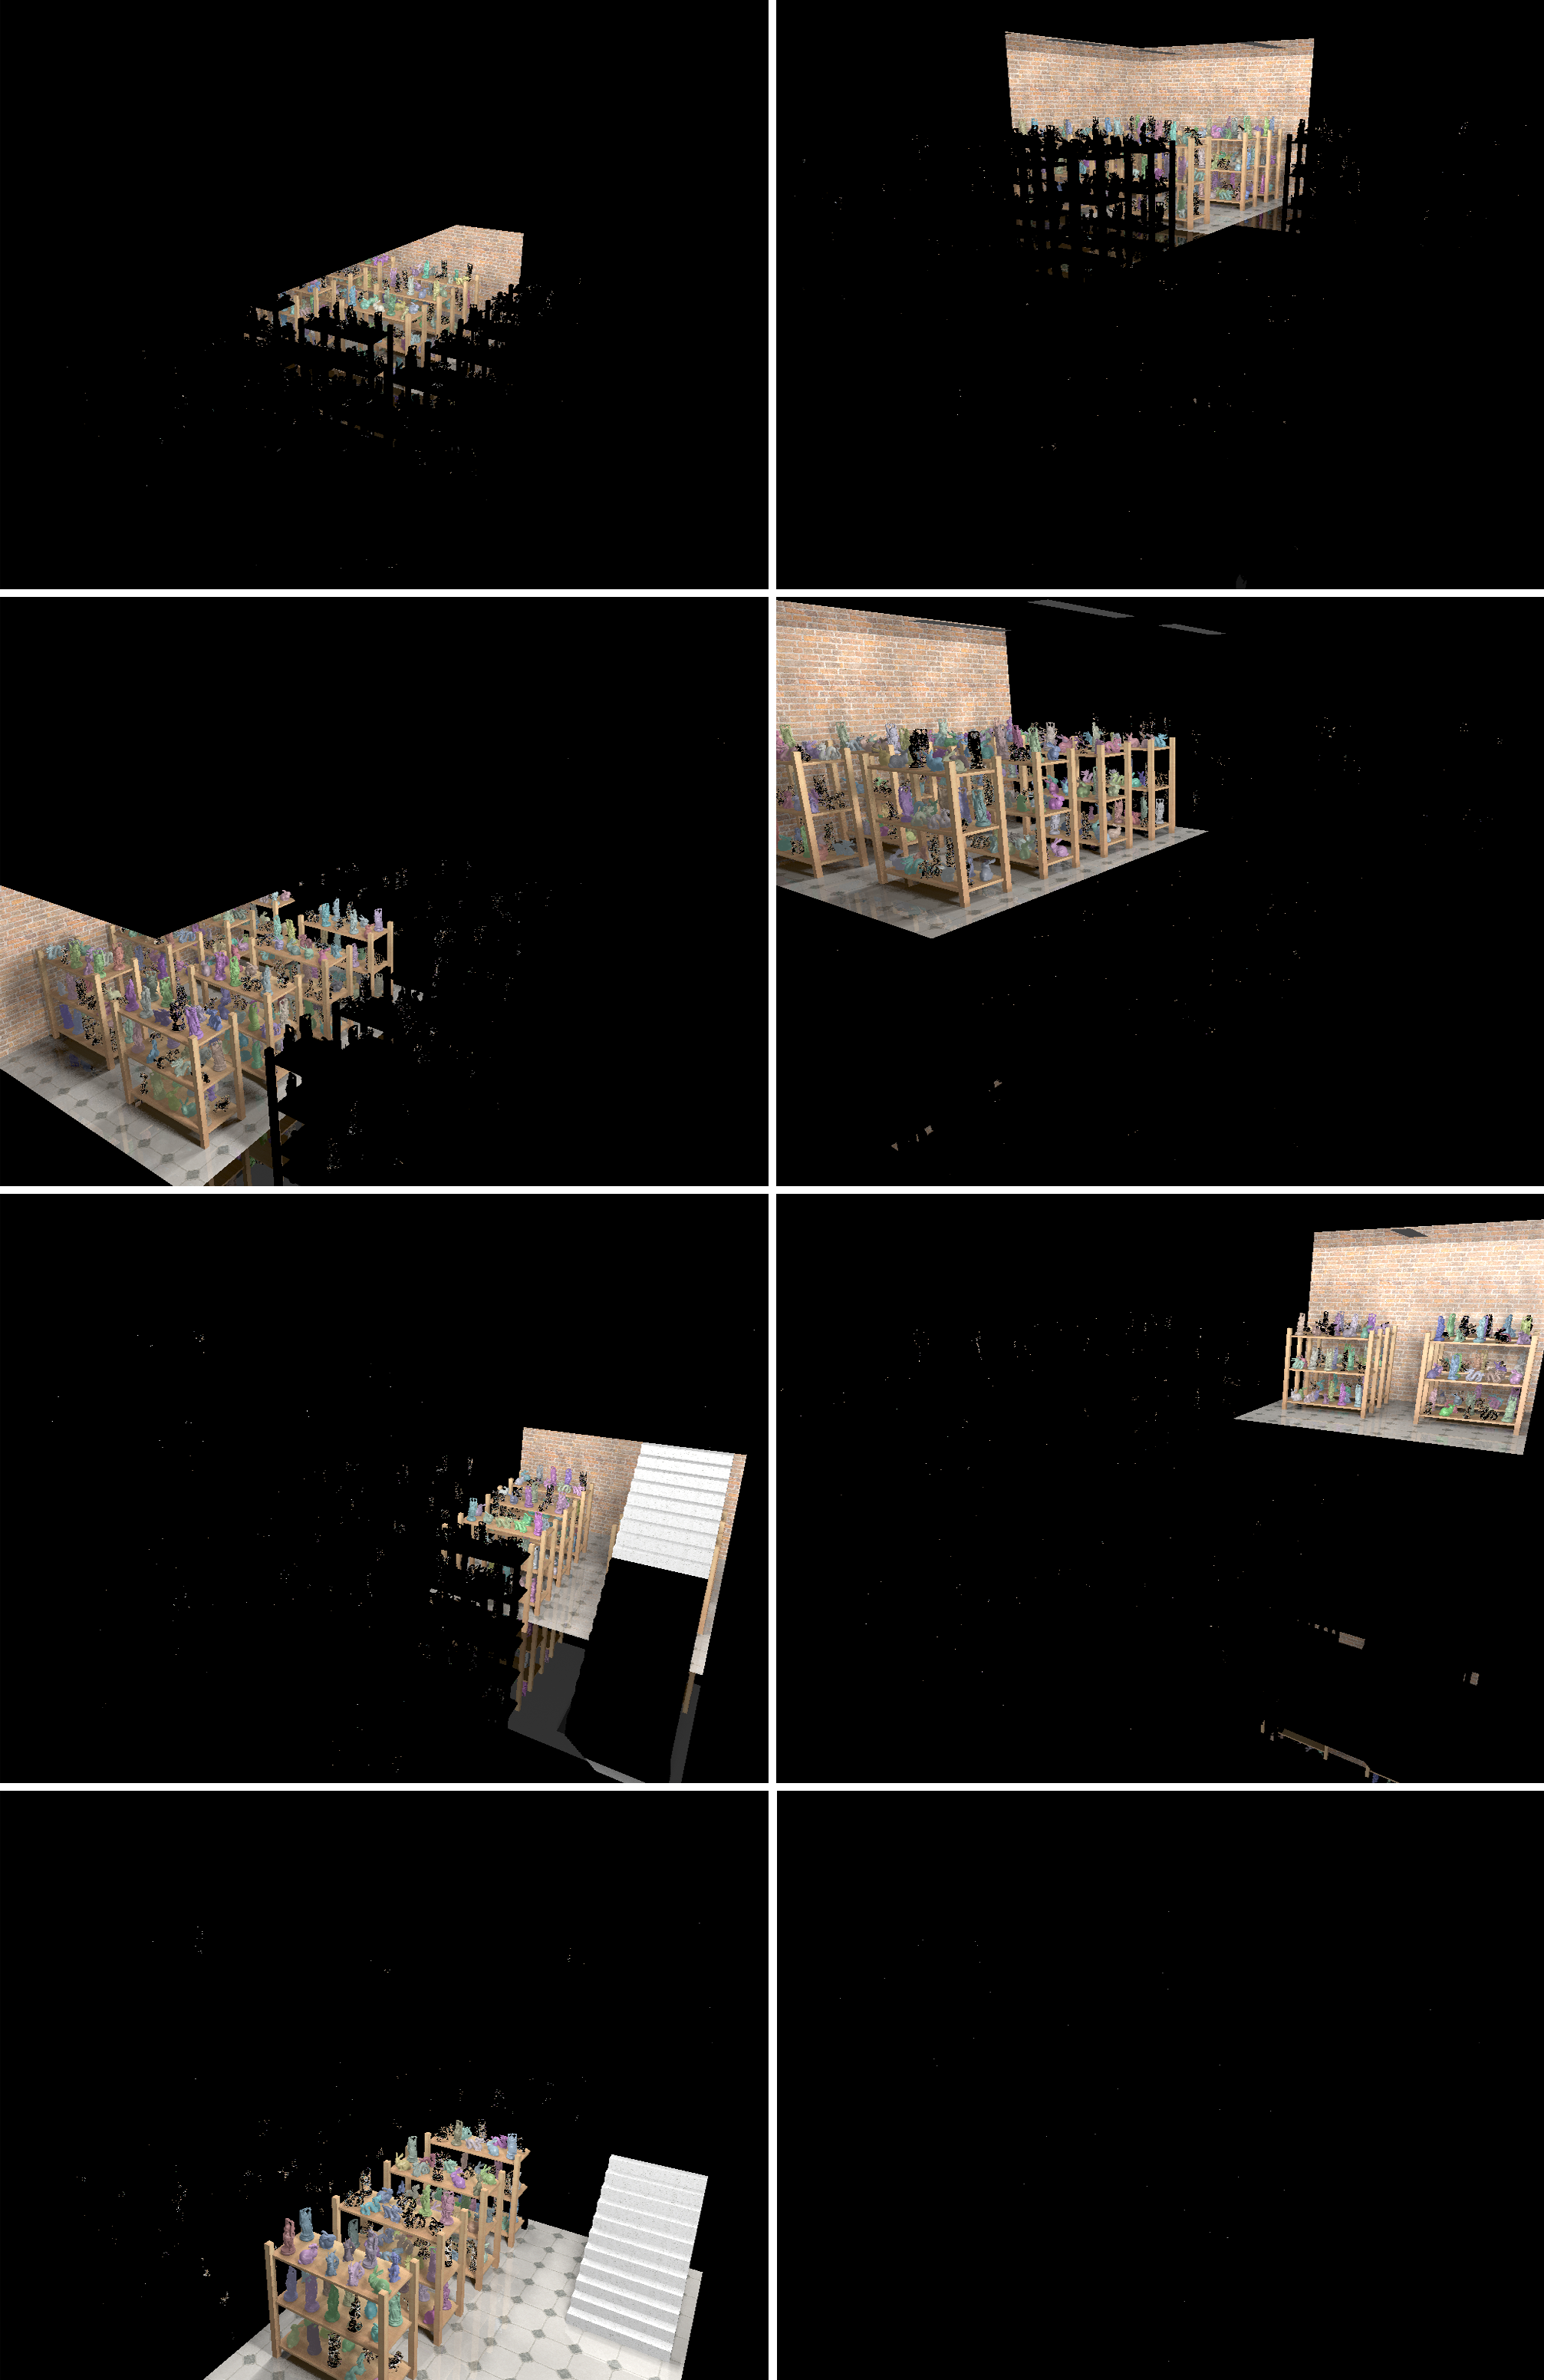
\includegraphics[width=80mm]{images/toystoredistribution.png}
%    \caption{The individual worker image buffers that are combined to form the final image.}
 %   \label{fig:toystoredist}
%\end{figure}

\subsection{Geometry Distribution}
\label{geomdist}

To ensure the entire scene stays in core, FlexRender must distribute the
geometry across the available RAM in the cluster effectively. With the exception
of one worker, the Morton coding and Z-order curve did a decent job of
partitioning the scene data evenly. See Figure~\ref{fig:geomdist} for a break down of the 
distribution of the geometry.  The one worker which did not contain very much geometry was in the top corner
of the Toy Store closest to the camera. This octant of the scene only contained
a fill light facing the rest of the geometry.

\begin{figure}[h!]
    \centering
    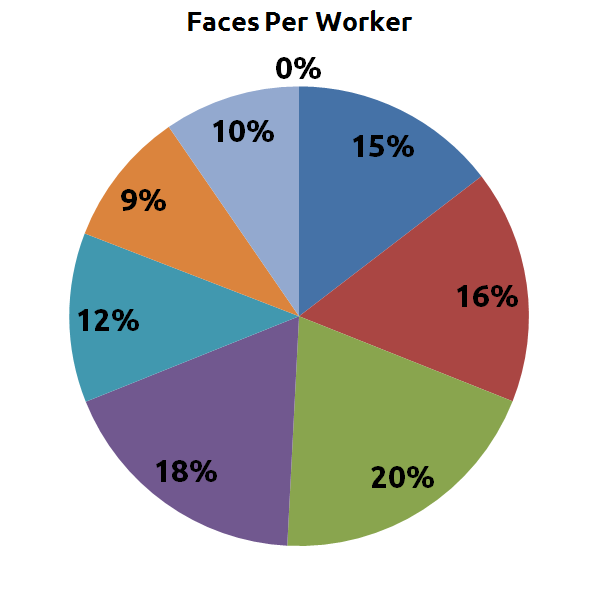
\includegraphics[width=50mm]{figures/facesperworker.png}
    \caption{Percentage of total geometry that was distributed to each worker using FlexRender.  Beside the worker with no geometry (top corner with only a fill light) the size of geometry per worker varied from 9\% with 106 MB of geometry data and 488 MB of BVH data to 20\% of the scene data with  221 MB of geometry and 1007 MB of BVH data.}
    \label{fig:geomdist}
\end{figure}



%\begin{table}
%\begin{center}
%\begin{tabular}{|l||c|c|c|c|c|c|c|c|}
%   \hline
%     & 1 & 2 & 3 & 4 & 5 & 6 & 7 & 8 \\
%     \hline
%     \hline
 %    (G) & 162 & 183 & 221 & 202 & 133 & 106 & 107 & 0 \\
%     \hline
%     (B) & 742 & 837 & 1007 & 922 & 607 & 486 & 488 & 0 \\
%     \hline
% \end{tabular}
% \caption{}
% \label{tb:geomsize}
% \end{center}
% \end{table}

\paragraph{Network Hops:}
The intent of the top-level BVH is to reduce network cost by only sending
a ray across the network when we know it ventures into that worker's region
of space. Since a BVH is a $O(log\;n)$ data structure, we expect that with 8
workers the average ray would be handled by 3 workers during its lifetime.

\begin{table}
\begin{center}
\begin{tabular}{|r||c|c|c|c|}
    \hline
    \# Workers& 1 & 2 & 3 & 4 \\

    \hline
    \% of Rays & 15.8\% & 25.6\% & 21.8\% & 18.8\%\\
\hline
        \hline
           \# Workers & 5 & 6 & 7 & 8+ \\
               \hline
                    \% of Rays    & 8.9\% & 7.4\% & 1.5\% & 0.2\% \\
    \hline
\end{tabular}
\caption{Percentage of rays that were processed by the given number of workers.}
\label{tb:nethopspercent}
\end{center}
\end{table}

Our results, see Table~\ref{tb:nethopspercent}, show that 63.2\% of rays are handled by 3 workers or less, and
nearly 16\% of them never even go out over the network (they are generated on,
intersect with, and are shaded on a single worker). We also see that 36.8\% of
rays must touch more than the expected 3 workers.  However, if we include the 
corner cases mentioned in \ref{traversal}, we see that
82\% of rays are at or below $O((log\;n) + 1)$ and 90.9\% of rays are at or
below $O((log\;n) + 2)$. 

\paragraph{Ray Queue Sizes}
Keeping the ray queue size small is critical to the long term health of the
render. If rays begin piling up faster than the cluster can process them,
eventually the cluster will begin swapping when accessing rays, which violates
our fundamental performance goal to stay off of disk.

Because of this, we benchmarked the ray queue sizes on each worker over time
when rendering Toy Store on a cluster of 16 workers. Figure \ref{fig:queuesize}
shows this with each renderer displayed as a different color. Table \ref{tb:rayqueues}
breaks down the average queue size, as well as the maximum size over the course
of the entire render and the storage requirements of the maximum size, both in
terms of raw storage space and a fraction of the system RAM.

As Table \ref{tb:rayqueues} shows, most workers sit comfortably below 1\% of
their RAM being used for queued rays, while the busiest worker used just over
1\%. This demonstrates that our regulation mechanisms and work throttling is
working well to keep the cluster from generating more work than it can handle.

\begin{figure}[h!]
    \centering
    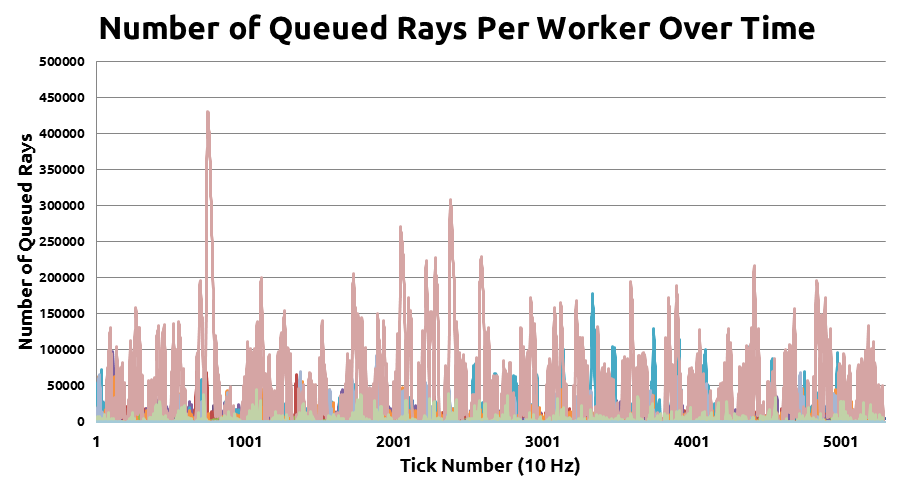
\includegraphics[width=70mm]{figures/queuesize.png}
    \caption{Number of rays queued on each worker over time. Different colors correspond to different workers.}
    \label{fig:queuesize}
\end{figure}

\begin{table}
\begin{center}
\begin{tabular}{|c||c|c|c|c|}
    \hline
    & Avg  & Max & Max & Memory \\
     & Queued & Queued & Storage & Use \\
    \hline
    \hline
    1 & 107 & 12221 & 1.49 MB & 0.04\% \\
    \hline
    2 & 506 & 29796 & 3.64 MB & 0.09\% \\
    \hline
    3 & 969 & 34970 & 4.27 MB & 0.10\% \\
    \hline
    4 & 3116 & 57597 & 7.03 MB & 0.17\% \\
    \hline
    5 & 1687 & 36981 & 4.51 MB & 0.11\% \\
    \hline
    6 & 1430 & 44053 & 5.38 MB & 0.13\% \\
    \hline
    7 & 4070 & 80899 & 9.88 MB & 0.24\% \\
    \hline
    8 & 2000 & 16861 & 2.06 MB & 0.05\% \\
    \hline
    9 & 3767 & 97429 & 11.89 MB & 0.29\% \\
    \hline
    10 & 7921 & 178191 & 21.75 MB & 0.53\% \\
    \hline
    11 & 4477 & 69702 & 8.51 MB & 0.21\% \\
    \hline
    12 & 4943 & 92043 & 11.24 MB & 0.27\% \\
    \hline
    13 & 51164 & 430736 & 52.58 MB & 1.28\% \\
    \hline
    14 & 2193 & 45428 & 5.55 MB & 0.14\% \\
    \hline
    15 & 0 & 0 & 0 MB & 0.00\% \\
    \hline
    16 & 18 & 1374 & 0.17 MB & 0.01\% \\
    \hline
\end{tabular}
\caption{Size of ray queues when rendering Toy Store with a 16-worker FlexRender cluster.}
\label{tb:rayqueues}
\end{center}
\end{table}

\paragraph{Cluster Size}
To evaluate the scalability of the FlexRender architecture, we ran Toy Store
renders with cluster sizes of 4 workers, 8 workers, and 16 workers. For
comparison, we ran the same renders in the traditional configuration also of
4, 8, and 16 workers.

As Table \ref{tb:clustersize} shows, we see a continual and impressive
improvement in the BVH construction time as the number of workers increases.
This is thanks to the huge parallelization speedup we get from partitioning
the scene geometry with Morton coding and building each subtree in parallel.

We also see render time improvements of roughly an order of magnitude, depending
on how FlexRender chooses to distribute the geometry based on the number of workers
available. It is likely that this performance advantage will slowly erode as the
cluster size grows larger (due to increasing network communication costs), but
for small to medium cluster sizes we see approximately linear growth.

\begin{table}
\begin{center}
\begin{tabular}{|l||c|c|c|}
    \hline
    \# Workers & 4 & 8  & 16  \\
    \hline
    \hline
    BVH Build & 203  & 184  & 171  \\
    \hline
    \emph{ flex BVH Build } & 39  & 20  & 10  \\
    \hline
    \textbf{(speedup)} & \textbf{5.21x} & \textbf{9.20x} & \textbf{17.1x} \\
    \hline
    \hline
    Render & 14833  & 10061  & 7702  \\
    \hline
    \emph{ flex Render}& 1742  & 1532  & 970  \\
    \hline
    \textbf{(speedup)} & \textbf{8.51x} & \textbf{6.57x} & \textbf{7.94x} \\
    \hline
    \hline
    Render  & 14536  & 9800  & 7413  \\
    w/o Load& &  &  \\
    \hline
    \emph{ flex Render} & 1405  & 1206  & 540  \\
    w/o Load& &  & \\
    \hline
    \textbf{(speedup)} & \textbf{10.35x} & \textbf{8.13x} & \textbf{13.73x} \\
    \hline
\end{tabular}
\caption{Comparison of cluster sizes with both the traditional configuration and the FlexRender configuration (in italics). All times shown are seconds.}
\label{tb:clustersize}
\end{center}
\end{table}

\paragraph{Example Renders}
Figure \ref{fig:sotoystore} shows the final Toy Store scene render, with 42 million
triangles and nearly 1,300 models.



Figure \ref{fig:sofield} shows a render with even higher resolution models,
bringing the geometric complexity up to 87 million triangles.



Figure \ref{fig:sodist} shows a monochromatic Cornell Box rendered by two workers.
The final composite is on the left, while the individual image buffers are on the right.
With only direct lighting and no reflections, this clearly demonstrates which
geometry was assigned to each worker.

\begin{figure}[h!]
    \centering
    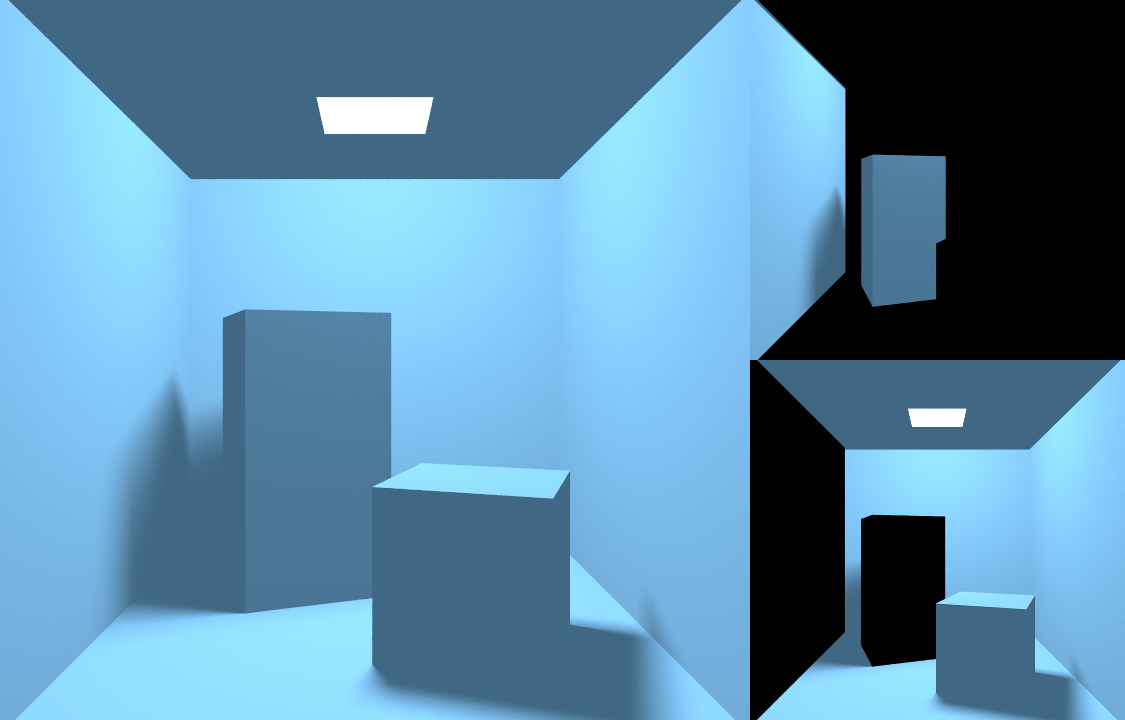
\includegraphics[width=80mm]{showoff/distribution.png}

    \caption{A monochromatic Cornell Box, showing the distribution of geometry between two workers.}
    \label{fig:sodist}
\end{figure}

Figure \ref{fig:socornell} demonstrates FlexRender's Lua-based shader system. The
Stanford bunny model is toon shaded, while the Buddha model has a perfect mirror
finish. Reflection rays for the mirrored Buddha and floor are cast directly
from the shaders.

\begin{figure}[h!]
    \centering
    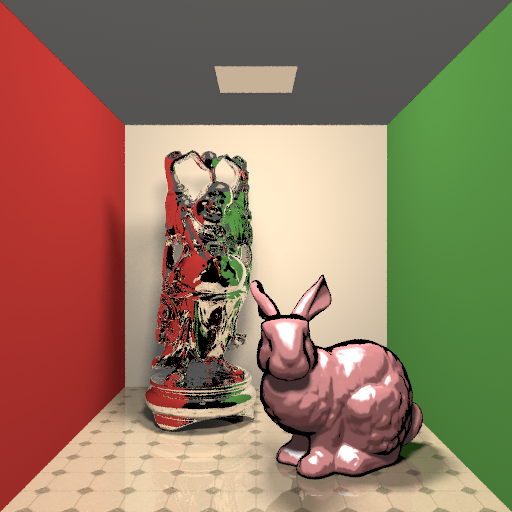
\includegraphics[width=80mm]{showoff/cornell-models.png}
    \caption{A Cornell Box with a toon shaded Stanford bunny and mirrored Buddha.}
    \label{fig:socornell}
\end{figure}

%Figure \ref{fig:sogi} shows an example of a Monte Carlo global illumination shader, as rendered by two workers. At first it appears that the geometry is present on all workers. However, the lighting tells the full story. The geometry is split the same way as in Figure \ref{fig:sodist}. Each worker image contains direct light for the geometry on that worker, as well as indirect light \emph{reflected by} geometry on that worker.

%\begin{figure}[h!]
  %  \centering
%    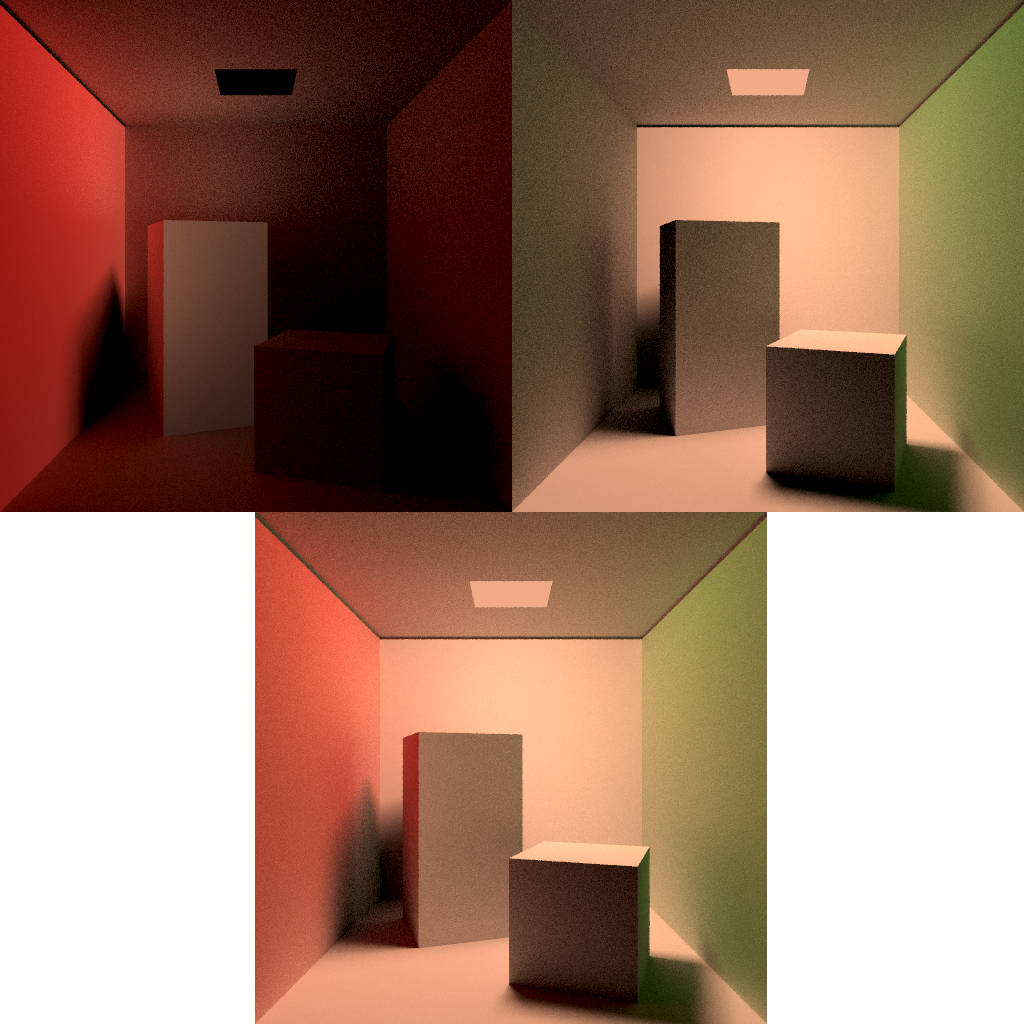
\includegraphics[width=80mm]{showoff/gi.png}
%    \caption{A Cornell Box with a Monte Carlo global illumination shader. The top row shows individual worker renders, the bottom center is the final composite. Each worker has direct light for the geometry on its machine and indirect light caused by the geometry on its machine.}
%    \label{fig:sogi}
%\end{figure}

\subsection{Summary}
\label{resultssummary}

With these results, we have demonstrated that FlexRender meets our claimed
contributions in the following ways. 

\begin{itemize}
    \item The scene geometry and acceleration structure data stays in-core due
        to effective scene distribution.
    \item Rays carry enough state to never require replies and the generated
        images match our baseline implementation.
    \item We can correctly and efficiently traverse the scene when workers
        only contain spatially local BVHs, linked by a top-level BVH.
    \item The top-level BVH effectively reduces the amount of network
        communication necessary to render the scene.
    \item The system keeps itself regulated and reduces memory usage by
        throttling new work generation and processing rays in an intelligent
        order.
    \item We show consistent speedups over the traditional approach, which
        suffers greatly from having to hit disk frequently during the
        rendering process.
\end{itemize}

\subsection{Future Work}
\label{futurework}

Currently there are two competing concerns in FlexRender. The first is to
distribute the scene data well, such that the geometry distribution is balanced
and everything is in-core. The second is to maximize
the utilization of the available processing power in the cluster. Unfortunately,
these concerns are somewhat at odds: good geometry distribution
is a result of distributing 3D space well, whereas good workload distribution
is a result of distributing screen space well. 
The Z-order curve works well for spatially uniform scenes, but unfortunately a
lot of scenes that are interesting to render are usually uniformly distributed
in image space, not 3D space. 
%In retrospect, we believe that the Morton coding and Z-order curve was a poor choice for the distribution of geometry. 
%It was initially chosen because we did not want to require a preprocessing (or \emph{baking}) step for determining the optimal distribution of geometry. 
%Since the scene was presumably too large to fit in core on any one machine, preprocessing the scene as a whole was deemed to be against the spirit of the problem.

One solution would be a quick prepassrendering. If we have information about the
layout of the scene in image space prior to rendering, we have some opportunities
for moving things around to adjust the workload before it becomes a problem during
rendering. A prepass render likewise could contribute to reducing extra network hops.
By gathering information about the
layout of the scene in image space and carefully choosing the slices of the
image that each worker was responsible for casting primary rays in, we could
dramatically increase the chances that the ray would intersect the geometry
on the worker and finish shading without ever touching the network. 

Some network hops could be avoided in the situation when the ray finishes
traversing the top-level BVH but ends up on a worker that is not the point of
intersection. Because the worker has no shading assets for that geometry, it
must pass the ray back to the ``winning'' worker for shading. By distributing
all of the shading assets (shaders, textures, and materials) to all workers,
any worker would be capable of shading a ray at the conclusion of its BVH traversal.

Potential memory optimizations could be based on the transient
nature of many fixed-size fat rays, which is a perfect opportunity to use an object
pool to reduce allocation overhead and heap fragmentation.
In addition, the linear BVH nodes structures were intentionally padded to
64-bytes to match the cache line size on current CPUs. However without a custom
STL allocator for the vector that stores this array of nodes, cache alignment
is not guaranteed. 

Finally, one of FlexRender's strengths is that it decouples the ray tracing computations
at the level of the individual ray. Because workers are never waiting on other workers for the results of a computation, this opens up the possibility for batching data to a GPU worker.
%Because workers in the cluster speak adefined network protocol to pass rays around, this opens the door for workers to join the cluster with new and interesting machine architectures.
%FlexRender's architecture is amiable to amortizing the cost of bus transfers in GPGPU computing.

%\vfill
\bibliographystyle{apalike}
{\small
\bibliography{RS_VISIGRAPP}}

\vfill
\end{document}

